%  A simple AAU report template.
%  2015-05-08 v. 1.2.0
%  Copyright 2010-2015 by Jesper Kjær Nielsen <jkn@es.aau.dk>
%
%  This is free software: you can redistribute it and/or modify
%  it under the terms of the GNU General Public License as published by
%  the Free Software Foundation, either version 3 of the License, or
%  (at your option) any later version.
%
%  This is distributed in the hope that it will be useful,
%  but WITHOUT ANY WARRANTY; without even the implied warranty of
%  MERCHANTABILITY or FITNESS FOR A PARTICULAR PURPOSE.  See the
%  GNU General Public License for more details.
%  TEST!
%  You can find the GNU General Public License at <http://www.gnu.org/licenses/>.
%

%  A simple AAU report template.
%  2015-05-08 v. 1.2.0
%  Copyright 2010-2015 by Jesper Kjær Nielsen <jkn@es.aau.dk>
%
%  This is free software: you can redistribute it and/or modify
%  it under the terms of the GNU General Public License as published by
%  the Free Software Foundation, either version 3 of the License, or
%  (at your option) any later version.
%
%  This is distributed in the hope that it will be useful,
%  but WITHOUT ANY WARRANTY; without even the implied warranty of
%  MERCHANTABILITY or FITNESS FOR A PARTICULAR PURPOSE.  See the
%  GNU General Public License for more details.
%
%  You can find the GNU General Public License at <http://www.gnu.org/licenses/>.
%
\documentclass[11pt,twoside,a4paper,openright]{report}
%%%%%%%%%%%%%%%%%%%%%%%%%%%%%%%%%%%%%%%%%%%%%%%%
% Language, Encoding and Fonts
% http://en.wikibooks.org/wiki/LaTeX/Internationalization
%%%%%%%%%%%%%%%%%%%%%%%%%%%%%%%%%%%%%%%%%%%%%%%%
% Select encoding of your inputs. Depends on
% your operating system and its default input
% encoding. Typically, you should use
%   Linux  : utf8 (most modern Linux distributions)
%            latin1 
%   Windows: ansinew
%            latin1 (works in most cases)
%   Mac    : applemac
% Notice that you can manually change the input
% encoding of your files by selecting "save as"
% an select the desired input encoding. 
\usepackage[utf8]{inputenc}
% Make latex understand and use the typographic
% rules of the language used in the document.
\usepackage[danish,english]{babel}
% Use the palatino font
\usepackage[sc]{mathpazo}
\linespread{1.05}         % Palatino needs more leading (space between lines)
% Choose the font encoding
\usepackage[T1]{fontenc}
%%%%%%%%%%%%%%%%%%%%%%%%%%%%%%%%%%%%%%%%%%%%%%%%
% Graphics and Tables
% http://en.wikibooks.org/wiki/LaTeX/Importing_Graphics
% http://en.wikibooks.org/wiki/LaTeX/Tables
% http://en.wikibooks.org/wiki/LaTeX/Colors
%%%%%%%%%%%%%%%%%%%%%%%%%%%%%%%%%%%%%%%%%%%%%%%%
% load a colour package
\usepackage{xcolor}
\definecolor{aaublue}{RGB}{33,26,82}% dark blue
% The standard graphics inclusion package
\usepackage{graphicx}
% Set up how figure and table captions are displayed
\usepackage{caption}
\captionsetup{%
  font=footnotesize,% set font size to footnotesize
  labelfont=bf % bold label (e.g., Figure 3.2) font
}
% Make the standard latex tables look so much better
\usepackage{array,booktabs}
% Enable the use of frames around, e.g., theorems
% The framed package is used in the example environment
\usepackage{framed}

%%%%%%%%%%%%%%%%%%%%%%%%%%%%%%%%%%%%%%%%%%%%%%%%
% Mathematics
% http://en.wikibooks.org/wiki/LaTeX/Mathematics
%%%%%%%%%%%%%%%%%%%%%%%%%%%%%%%%%%%%%%%%%%%%%%%%
% Defines new environments such as equation,
% align and split 
\usepackage{amsmath}
% Adds new math symbols
\usepackage{amssymb}
% Use theorems in your document
% The ntheorem package is also used for the example environment
% When using thmmarks, amsmath must be an option as well. Otherwise \eqref doesn't work anymore.
\usepackage[framed,amsmath,thmmarks]{ntheorem}

%%%%%%%%%%%%%%%%%%%%%%%%%%%%%%%%%%%%%%%%%%%%%%%%
% Page Layout
% http://en.wikibooks.org/wiki/LaTeX/Page_Layout
%%%%%%%%%%%%%%%%%%%%%%%%%%%%%%%%%%%%%%%%%%%%%%%%
% Change margins, papersize, etc of the document
\usepackage[
  inner=28mm,% left margin on an odd page
  outer=41mm,% right margin on an odd page
  ]{geometry}
% Modify how \chapter, \section, etc. look
% The titlesec package is very configureable
\usepackage{titlesec}
\titleformat{\chapter}[display]{\normalfont\huge\bfseries}{\chaptertitlename\ \thechapter}{20pt}{\Huge}
\titleformat*{\section}{\normalfont\Large\bfseries}
\titleformat*{\subsection}{\normalfont\large\bfseries}
\titleformat*{\subsubsection}{\normalfont\normalsize\bfseries}
%\titleformat*{\paragraph}{\normalfont\normalsize\bfseries}
%\titleformat*{\subparagraph}{\normalfont\normalsize\bfseries}

% Clear empty pages between chapters
\let\origdoublepage\cleardoublepage
\newcommand{\clearemptydoublepage}{%
  \clearpage
  {\pagestyle{empty}\origdoublepage}%
}
\let\cleardoublepage\clearemptydoublepage

% Change the headers and footers
\usepackage{fancyhdr}
\pagestyle{fancy}
\fancyhf{} %delete everything
\renewcommand{\headrulewidth}{0pt} %remove the horizontal line in the header
\fancyhead[RE]{\small\nouppercase\leftmark} %even page - chapter title
\fancyhead[LO]{\small\nouppercase\rightmark} %uneven page - section title
\fancyhead[LE,RO]{\thepage} %page number on all pages
% Do not stretch the content of a page. Instead,
% insert white space at the bottom of the page
\raggedbottom
% Enable arithmetics with length. Useful when
% typesetting the layout.
\usepackage{calc}

%%%%%%%%%%%%%%%%%%%%%%%%%%%%%%%%%%%%%%%%%%%%%%%%
% Bibliography
% http://en.wikibooks.org/wiki/LaTeX/Bibliography_Management
%%%%%%%%%%%%%%%%%%%%%%%%%%%%%%%%%%%%%%%%%%%%%%%%
\usepackage[backend=bibtex,
  bibencoding=utf8
  ]{biblatex}
\addbibresource{bib/mybib}

%%%%%%%%%%%%%%%%%%%%%%%%%%%%%%%%%%%%%%%%%%%%%%%%
% Misc
%%%%%%%%%%%%%%%%%%%%%%%%%%%%%%%%%%%%%%%%%%%%%%%%
% Add bibliography and index to the table of
% contents
\usepackage[nottoc]{tocbibind}
% Add the command \pageref{LastPage} which refers to the
% page number of the last page
\usepackage{lastpage}
% Add todo notes in the margin of the document
\usepackage[
%  disable, %turn off todonotes
  colorinlistoftodos, %enable a coloured square in the list of todos
  textwidth=\marginparwidth, %set the width of the todonotes
  textsize=scriptsize, %size of the text in the todonotes
  ]{todonotes}

%%%%%%%%%%%%%%%%%%%%%%%%%%%%%%%%%%%%%%%%%%%%%%%%
% Hyperlinks
% http://en.wikibooks.org/wiki/LaTeX/Hyperlinks
%%%%%%%%%%%%%%%%%%%%%%%%%%%%%%%%%%%%%%%%%%%%%%%%
% Enable hyperlinks and insert info into the pdf
% file. Hypperref should be loaded as one of the 
% last packages
\usepackage{hyperref}
\hypersetup{%
	pdfpagelabels=true,%
	plainpages=false,%
	pdfauthor={Author(s)},%
	pdftitle={Title},%
	pdfsubject={Subject},%
	bookmarksnumbered=true,%
	colorlinks=false,%
	citecolor=black,%
	filecolor=black,%
	linkcolor=black,% you should probably change this to black before printing
	urlcolor=black,%
	pdfstartview=FitH%
}
% package inclusion and set up of the document
%!TEX root = ../master.tex
% see, e.g., http://en.wikibooks.org/wiki/LaTeX/Formatting#Hyphenation
% for more information on word hyphenation
\hyphenation{ex-am-ple hy-phen-a-tion short}
\hyphenation{long la-tex}
% 
%!TEX root = ../master.tex
%  A simple AAU report template.
%  2015-05-08 v. 1.2.0
%  Copyright 2010-2015 by Jesper Kjær Nielsen <jkn@es.aau.dk>
%
%  This is free software: you can redistribute it and/or modify
%  it under the terms of the GNU General Public License as published by
%  the Free Software Foundation, either version 3 of the License, or
%  (at your option) any later version.
%
%  This is distributed in the hope that it will be useful,
%  but WITHOUT ANY WARRANTY; without even the implied warranty of
%  MERCHANTABILITY or FITNESS FOR A PARTICULAR PURPOSE.  See the
%  GNU General Public License for more details.
%
%  You can find the GNU General Public License at <http://www.gnu.org/licenses/>.
%
%
%
% see, e.g., http://en.wikibooks.org/wiki/LaTeX/Customizing_LaTeX#New_commands
% for more information on how to create macros

%%%%%%%%%%%%%%%%%%%%%%%%%%%%%%%%%%%%%%%%%%%%%%%%
% Macros for the titlepage
%%%%%%%%%%%%%%%%%%%%%%%%%%%%%%%%%%%%%%%%%%%%%%%%
%Creates the aau titlepage
\newcommand{\aautitlepage}[3]{%
  {
    %set up various length
    \ifx\titlepageleftcolumnwidth\undefined
      \newlength{\titlepageleftcolumnwidth}
      \newlength{\titlepagerightcolumnwidth}
    \fi
    \setlength{\titlepageleftcolumnwidth}{0.5\textwidth-\tabcolsep}
    \setlength{\titlepagerightcolumnwidth}{\textwidth-2\tabcolsep-\titlepageleftcolumnwidth}
    %create title page
    \thispagestyle{empty}
    \noindent%
    \begin{tabular}{@{}ll@{}}
      \parbox{\titlepageleftcolumnwidth}{
        \iflanguage{danish}{%
          
\includegraphics[width=\titlepageleftcolumnwidth]{figures/aau_logo_da}
        }{%
          
\includegraphics[width=\titlepageleftcolumnwidth]{figures/aau_logo_en}
        }
      } &
      \parbox{\titlepagerightcolumnwidth}{\raggedleft\sf\small
        #2
      }\bigskip\\
       #1 &
      \parbox[t]{\titlepagerightcolumnwidth}{%
      \textbf{Abstract:}\bigskip\par
        \fbox{\parbox{\titlepagerightcolumnwidth-2\fboxsep-2\fboxrule}{%
          #3
        }}
      }\\
    \end{tabular}
    \vfill
    \iflanguage{danish}{%
      \noindent{\footnotesize\emph{Rapportens indhold er frit tilgængeligt, men offentliggørelse (med kildeangivelse) må kun ske efter aftale med forfatterne.}}
    }
    \clearpage
  }
}

%Create english project info
\newcommand{\englishprojectinfo}[8]{%
  \parbox[t]{\titlepageleftcolumnwidth}{
    \textbf{Title:}\\ #1\bigskip\par
    \textbf{Theme:}\\ #2\bigskip\par
    \textbf{Project Period:}\\ #3\bigskip\par
    \textbf{Project Group:}\\ #4\bigskip\par
    \textbf{Participant(s):}\\ #5\bigskip\par
    \textbf{Supervisor(s):}\\ #6\bigskip\par
    \textbf{Copies:} #7\bigskip\par
    \textbf{Page Numbers:} 69 \bigskip\par
    \textbf{Date of Completion:}\\ #8
  }
}

%Create danish project info
\newcommand{\danishprojectinfo}[8]{%
  \parbox[t]{\titlepageleftcolumnwidth}{
    \textbf{Titel:}\\ #1\bigskip\par
    \textbf{Tema:}\\ #2\bigskip\par
    \textbf{Projektperiode:}\\ #3\bigskip\par
    \textbf{Projektgruppe:}\\ #4\bigskip\par
    \textbf{Deltager(e):}\\ #5\bigskip\par
    \textbf{Vejleder(e):}\\ #6\bigskip\par
    \textbf{Oplagstal:} #7\bigskip\par
    \textbf{Sidetal:} 69\bigskip\par
    \textbf{Afleveringsdato:}\\ #8
  }
}

%%%%%%%%%%%%%%%%%%%%%%%%%%%%%%%%%%%%%%%%%%%%%%%%
% An example environment
%%%%%%%%%%%%%%%%%%%%%%%%%%%%%%%%%%%%%%%%%%%%%%%%
\theoremheaderfont{\normalfont\bfseries}
\theorembodyfont{\normalfont}
\theoremstyle{break}
\def\theoremframecommand{{\color{gray!50}\vrule width 5pt \hspace{5pt}}}
\newshadedtheorem{exa}{Example}[chapter]
\newenvironment{example}[1]{%
		\begin{exa}[#1]
}{%
		\end{exa}
}
% my new macros

\begin{document}
%frontmatter
\pagestyle{empty} %disable headers and footers
\pagenumbering{roman} %use roman page numbering in the frontmatter
\graphicspath { {./figures/} }
%!TEX root = ../master.tex
%  A simple AAU report template.
%  2015-05-08 v. 1.2.0
%  Copyright 2010-2015 by Jesper Kjær Nielsen <jkn@es.aau.dk>
%
%  This is free software: you can redistribute it and/or modify
%  it under the terms of the GNU General Public License as published by
%  the Free Software Foundation, either version 3 of the License, or
%  (at your option) any later version.
%
%  This is distributed in the hope that it will be useful,
%  but WITHOUT ANY WARRANTY; without even the implied warranty of
%  MERCHANTABILITY or FITNESS FOR A PARTICULAR PURPOSE.  See the
%  GNU General Public License for more details.
%
%  You can find the GNU General Public License at <http://www.gnu.org/licenses/>.
%
\pdfbookmark[0]{Front page}{label:frontpage}%
\begin{titlepage}
  \addtolength{\hoffset}{0.5\evensidemargin-0.5\oddsidemargin} %set equal margins on the frontpage - remove this line if you want default margins
  \noindent%
  \begin{tabular}{@{}p{\textwidth}@{}}
    \toprule[2pt]
    \midrule
    \vspace{0.2cm}
    \begin{center}
    \Huge{\textbf{
      Report Title% insert your title here
    }}
    \end{center}
    \begin{center}
      \Large{
        - Subtitle -% insert your subtitle here
      }
    \end{center}
    \vspace{0.2cm}\\
    \midrule
    \toprule[2pt]
  \end{tabular}
  \vspace{4 cm}
  \begin{center}
    {\large
      Project Report%Insert document type (e.g., Project Report)
    }\\
    \vspace{0.2cm}
    {\Large
      MTA15341%Insert your group name or real names here
    }
  \end{center}
  \vfill
  \begin{center}
  Aalborg University\\
  Medialogy
  \end{center}
\end{titlepage}
\clearpage

\thispagestyle{empty}
{\small
\strut\vfill % push the content to the bottom of the page
\noindent Copyright \copyright{} Aalborg University 2015\par
\vspace{0.2cm}
\noindent{\footnotesize\emph{The content of this report is freely available, but publication (with reference) may only be pursued due to agreement with the author.}}
}
\clearpage


\pdfbookmark[0]{English title page}{label:titlepage_en}
\aautitlepage{%
  \englishprojectinfo{
    Augmented Boardgame %title
  }{%
    Visual Computing-Human Perception %theme
  }{%
    Autumn Semester 2015 %project period
  }{%
    MTA15341 % project group
  }{%
    %list of group members
    Daniel Vilcapaza\\ 
    Emilie Lind Damkjær\\
    Liv Arleth\\
    Markus Kristian Oerbæk Bertelsen\\
    Peter Kejser Jensen\\
    Rasmus Kaasgaard Christiansen
  }{%
    %list of supervisors
    Andreas Moegelmose
    
  }{%
    1 % number of printed copies
  }{%
    \today % date of completion
  }%
}{%department and address
  \textbf{Medialogy}\\
  Aalborg University\\
  \href{http://www.aau.dk}{http://www.aau.dk}
}{% the abstract
  Here is the abstract
}


\cleardoublepage
\pdfbookmark[0]{Contents}{label:contents}
\pagestyle{fancy} %enable headers and footers again
\tableofcontents
%!TEX root = ../master.tex
\chapter*{Glossary}\label{gloss}

\textbf{RDI}: Rear Diffused Illumination is the name of a solution of a multi-touch device\citep{multiTT}. This solution has an optical sensor, which in infra-red captures the contrast between a silent image and objects touching the surface.

\textbf{LED}: Light-emitting diode, which glows when voltage is applied to it, like for example a light bulb.

\textbf{IR}: Infra-red, which is radiant energy that is invisible to the human eye, due to it being of lower frequency and larger wavelength than visible light.

\textbf{BLOB}: Binary Large Object, which is an object made up from connected pixels in an binary image. 

\textbf{Terraforming}: A game mechanic in Terra Mystica, where the player changes a tile in the game into a tile that he can place game pieces on. This is necessary, since each player can only place game pieces on one kind of terrain.

\textbf{Power}: A currency in the game Terra Mystica which is used to do certain actions.

\textbf{LCD}: "LCD (liquid crystal display) is the technology used for displays in notebook and other smaller computers. Like light-emitting diode (LED) and gas-plasma technologies, LCDs allow displays to be much thinner than cathode ray tube (CRT) technology." \todo{directly quoted from google search "lcd means}
%\listoftodos
%\chapter*{Preface\markboth{Preface}{Preface}}\label{ch:preface}
\addcontentsline{toc}{chapter}{Preface}
Here is the preface. You should put your signatures at the end of the preface.

\vspace{\baselineskip}\hfill Aalborg University, \today
\vfill\noindent
\begin{minipage}[b]{0.45\textwidth}
 \centering
 \rule{\textwidth}{0.5pt}\\
  Author 1\\
 {\footnotesize <username1@XX.aau.dk>}
\end{minipage}
\hfill
\begin{minipage}[b]{0.45\textwidth}
 \centering
 \rule{\textwidth}{0.5pt}\\
  Author 2\\
 {\footnotesize <username2@XX.aau.dk>}
\end{minipage}
\vspace{3\baselineskip}
\begin{center}
\begin{minipage}[b]{0.45\textwidth}
 \centering
 \rule{\textwidth}{0.5pt}
  Author 3\\
 {\footnotesize <username3@XX.aau.dk>}
\end{minipage}
\end{center}

\cleardoublepage
%mainmatter
\pagenumbering{arabic} %use arabic page numbering in the mainmatter
%!TEX root = ../master.tex
\chapter{Introduction}\label{ch:introduction}

Board games come in many shapes, sizes, and levels of complexity. While some people see complexity as a pleasant challenge, others find it to be overwhelming, and therefore are these games intimidating to play. This is due to the players themselves are the only ones that can make sure that the game is being played according to the rules.

By incorporating computer-controlled elements into the board game, this project attempts to digitise and automate parts of it. This is to investigate, if a partly digitisation of the game can maintain the experience and enjoyment of play, while having certain parts handled by a computer.




\chapter{Initial Problem}\label{ch:ch2label}
Here we will explain our initial ideas and criteria we based our choices on.

We have based our initial problem formulation on our semester theme and our chosen project recommendation. Because of this, we wanted our initial problem formulation to be based on computer vision and a augmented board game, with the augmentation being based on computer vision. As we tried to specify what our analysis of the initial problem formulation should cover, we generated several ideas through brainstorming.

Those ideas each had a chosen board game, chosen technology needed for the ideas and a rough project process planning. Furthermore, all the ideas went through some criteria, in order to filter our ideas.
The criteria were:
\begin{enumerate}
	\item The idea must implement computer vision, since that is what we will need to fulfil our curriculum.
	\item The idea must include a existing board game that we have access to. So we do not design our own board game from scratch.
	\item The implemented computer vision for the idea must be interactive. This was important for us to remember, in order to stick with the main course of 3rd semester in the curriculum.
	\item The playtime of the idea's chosen board game must not have an average game time over two hours. This criteria was based on the assumption that if the game's playtime was too long, it would be harder to test it properly.
	\item The implemented computer vision may not make the board game itself more convoluted than it is. This criteria was added after a discussion, where the study group agreed on that we would not want to make the board games 'harder to play' than they were. ((maybe elaboration of rewording needed here).
\end{enumerate}

((Here there should be a list over our project ideas. I an not sure of what level of details are needed here, and how much of it should be in the appendix instead of this chapter - also, maybe there should even be a small detailed description of Terra mystica...not written by me))

The chosen project idea were a interactive board for the game Terra Mystica. We believed that such a project would require a projection of the board, while an implementation computer vision should detect physical game pieces on top of the board.
Our understanding of our chosen project idea lead us to make up an assumption of which things we would need to do in order to make our idea a reality:
\begin{enumerate}
\item First, we would need to make up the board for the projection. Here we imagined that the board's function and usability (project-wise)would be prioritised over cosmetics. We would then need to make the board a projection.
\item We then need the implemented computer vision to recognise the hexes that from a projected Terra Mystica board.
\item After that, the projected board must be able to change the colors of the hexes in it, since that is an essential visual part of the game itself.
\item The computer vision now needs to recognise the game pieces.
\item Now that the hexes can be recognised and change color while the game pieces also are being recognised, we will need to write/code(??!?) a program that can tie the hex color change to the game piece placement.
\end{enumerate}
%!TEX root = ../master.tex
\chapter{Background Research}\label{ch:bgres}
\todo{introduction to this chapter is needed. It needs an explanation to why this chapter is relevant}
The background research in this chapter is based on acquiring answers to the initial problem statement and the two research questions. The research includes studies of state of the art artefacts, previous work and which methods they used. 


\section{Target Group Explained}
The project's target group are people who are experienced with board games, maybe even Terra Mystica and are 14 years old or above since this is the game's recommended age group. This is because Terra Mystica itself caters to people who have a certain amount of experience with board games or people who like to play complex games, as the game has a lot of rules to keep track of. The project does not aim to simplify the game's core, but rather streamline the game mechanics, and therefore players who are inexperienced with complex board games will not benefit, since Terra Mystica is not a simple game to play.



\section{Previous scientific work}
In this section, other attempts to digitally augment board games will be discussed.

Andersen et al. \citep{andersen_designing_2004} created "BattleBoard3D", a board game utilising physical and digital components. For their physical components they used flat squares with patterns that through Augmented Reality (AR) technologies will be recognised through a camera and/or Virtual Reality goggles. Their research was made to illustrate "design issues for AR board games".

Peitz et al. \citep{peitzWizards2006} created "Wizard's Apprentice", a computer-augmented board game. The game includes two roles: wizard and apprentice. All players but one play as apprentices guided by the wizard who acts as a negotiator and motivator. The software is written in Java and has several play modes. The game uses Radio-Frequency Identification (RFID) hardware to detect at which physical point the players are in the game. It sends this information through antennas to a laptop close by. The laptop projects this information to a screen that displays relevant information on each player's turn. The game board can be seen in Figure \ref{fig:peitz}.

Magerkurth et al. \citep{magStars} created "STARS", a ubiquitous computing platform for computer augmented tabletop games. This platform includes devices such as a game table, a wall display, PDAs, and audio devices. The purpose of this platform was to provide features that went beyond what normal board games are capable of, while still maintaining the experience of the players interacting as they would with a normal board game. The platform was also able to save game states with ID tags, remember complex rules so they would not slow down the pacing of a game, and make the game board react dynamically to interactions with the game and its pieces. Its software is developer-friendly so that creating rules and content could be prioritised over device integration and game board management. 

\begin{figure}[!h]
\centering	
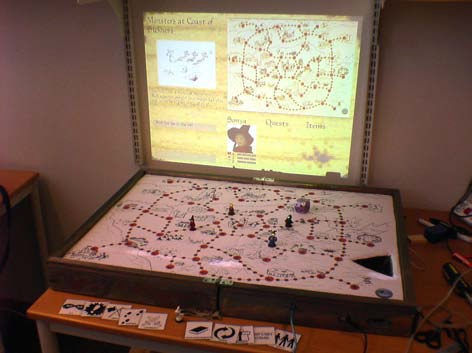
\includegraphics[width=0.5\textwidth]{peitz}
\caption{The Wizard's apprentice game board setup from \citep{peitzWizards2006}}
\label{fig:peitz}
\end{figure}

\section{Commercial competition}
Apart from previous scientific work, commercial board games have been released, existing on a spectrum ranging from completely digital to completely analogue. As our product will exist somewhere on the spectrum, these commercial solutions described below can be considered state of the art for this project.

\todo{do we need refs for these?}On the digital end, the online collectible card game Hearthstone (for Windows, OS X, Android and iOS), though completely virtual, has an interface which resembles a physical game board with cards and information on it. The user plays the game by dragging the cards onto the board from their 'hand' by way of using the cursor (when playing on a desktop computer), or by swiping with a finger (when playing on a smartphone or a tablet). The cards placed on the board can then be dragged to the cards they need to attack, etc. This swiping mechanism gives the game a tangible sense, making it resemble an analogue card game, even though no physical cards are involved.

There are also board games which integrate phone or tablet applications into the gameplay. One such game is XCOM: The Board Game, which simulates an alien attack the players then have to repel. The game has a physical game board, cards and pieces, but also a companion app, which can be downloaded to a desktop computer or mobile device. The app is required in order to play the game. It tracks the time each player has to do certain tasks, as well as what actions the aliens will take. The game therefore still looks like a normal board game, but it has a built-in augmentation in the form of the app, which changes the way turn/task orders and time constraints are done in a board game.

Another example of a board game which incorporates digital media is the card game, Munchkin. The game itself is a card game that can be played without augmentation. However, an app has been released which assists a player in keeping track of their current level and their combat strength compared to the monster they're fighting. Apart from that, the app provides the player using it with a bonus in the game. This is an example of a board game which has an optional digital augmentation, but it is not necessary to play the game.

\section{Methods for evaluating and measuring key success criteria}
Andersen et al. \citep{andersen_designing_2004} evaluated their product on a group of 13 year old children. The goals were to "reveal issues concerning the game design in general, design of the physical pieces, the use of goggles versus screen display, and future evolvement." The children found the 3D projection of the characters through the goggles fascinating, although some fumbling with the game pieces occurred due to the nature of the goggles and placement of the webcam. This occurred less when they looked at the 3D figures on the screen, but this brought along the problem of shifting focus away from the board game.
Finally, the children found the small set of animations uninteresting after a while and suggested a higher number of animations were needed to keep interest.

Peitz et al. \citep{peitzWizards2006} performed an initial evaluation on 3 children aged 8-9 and a male adult player (37). The evaluation was based upon a template that evaluates the social adaptability of game divided into: "(...)spatial, temporal, social, and playability." The participants were observed for two hours and were thematically interviewed afterwards. The participants reported overall enjoyment and increased togetherness in the game, but the pacing of the game felt unfamiliar. The participants seemed to particularly react positively to the sound design. 

\section{Competitive analysis}
As shown by Andersen et al. \citep{andersen_designing_2004}, a solution to enhance a board game can be done through AR aided by either a screen or Virtual Reality (VR) goggles. Andersen et al. mention some drawbacks to both of their technologies. In the case of AR with a screen they note that while the screen gives the participants the ability to look their opponent in the eye, they are distracted by having to look away from the board game space, to look at the screen displaying the figures. Regarding the VR, they note that participants liked the ability to pick up a game piece and explore all sides of the 3D model through the goggles. The problem, as can be seen in Figure \ref{fig:andersen}, could be that the goggles take away from the non-verbal communication that board games tend to foster.

In \citep{peitzWizards2006}, Peitz et al. built a board together with RFID antennas and other hardware to detect certain points of the the players' progression. They note some positive things, as aforementioned, namely the increased feeling of togetherness and overall enjoyment. They follow a recipe many traditional board games follow: a tile progression. They simulate this with the dots throughout the map, which the "tokens" press down on and activate. They also note the relationship between wizard and apprentices works well, but note an interesting development in the dynamics when one of the children effectively demotes the adult, who has the role as wizard, and temporarily acts as a new wizard. They did not account for this, but mention it is within their design goals.

As for the commercial competition, the solutions utilise digital media to varying degrees, in some cases combining these elements with traditional board game elements such as a board or cards, bringing in the aforementioned feeling of togetherness identified by Peitz et al \citep{peitzWizards2006}. However, in these multi-media solutions, the digital aspects are not integrated physically into the game, but rather exist as additional, separate 'piece' of the game in the form of a phone, tablet for personal computer. There is an unutilised potential in combining digital and physical elements in such a way that the players can feel the unity board games provide without the barrier of a screen between them, but at the same time have a program handle some of the management of parts, reducing the amount of time players have to spend on that.

\begin{figure}[!h]
\centering	
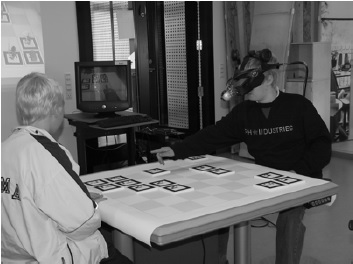
\includegraphics[width=0.5\textwidth]{andersen}
\caption{BattleBoard3D setup from Andersen et al.  \citep{andersen_designing_2004}}
\label{fig:andersen}
\end{figure}


\section{Terra Mystica}
Terra Mystica is a game that utilise a lot of different game pieces for different tasks. One of the tasks that use a lot of pieces is the task of terraforming a terrain into the factions home terrain. In some games a player can terraform so much that he/she runs out of pieces to terraform with. This problem could be solved though an interactive board, that removes the terrain pieces, and instead just changes the board itself. This way there is no way to run out of terraforming pieces.

\textbf{Power}

A mechanic often forgotten in the game is that when you build next to another player, you have to offer that player a thing called power, based on which building are adjacent to the build you just placed, and if the power value is above one, you lose victory points based on power value minus one. With an augmentation it would be possible for the game to tell the players involved in the offering of power, to just get a notice that tells them exactly how much power they would gain, and how many victory points they would lose on it.

\textbf{Cult track}

Terra Mystica has a mechanic called the cult track, which is a separate board with four different cults on it, as the game progresses players may gain cult points which grants them power, and in the end of the game, the players with the highest,second highest, and third highest value in the cult track gains additional points based on their position. Through an augmentation to the game it would be possible to make the cult track a program, that kept track of who was where, and who was winning the different tracks. 
%!TEX root = ../master.tex
\chapter{Final Problem}\label{ch:finprob}
The initial problem formulation provided research questions to expand our understanding of the problem area. The following final problem formulation is instead focused on the development of our product.

\section{Formulation}
After having chosen Terra Mystica as the board game to augment, the augmentation was decided as being an interactive game board via computer vision.

The initial research questions were:
\begin{itemize}
	\item How can computer vision be used to facilitate user interaction?
	\item How should the software for that be developed?
\end{itemize}

As seen in previous scientific work with examples of current state of the art, Andersen et al. \citep{andersen_designing_2004} used recognition technology via camera and Peitz et al. \citep{peitzWizards2006} showed the output from a game unto a projection. Both can add inspiration to how the initial research questions may be answered. An example being, creating an interactive projection, and having it being manipulated through interaction with its computer vision software.

The results of the ensuing background research were that BLOB recognition and background imaging in an RID solution would be a possible facilitation.
The software for that should be designed in such a way that the user can:
\begin{itemize}
\item Control the turn order
\item Start and end their own turn
\item Change a tile on the screen by 'terraforming'
\end{itemize}

In this project, an unutilised potential was identified when researching how augmentation like the current project idea would affect the usability of the game, in comparison to the non-augmented version. All that culminates into the final problem formulation:

\textit{“Can Terra Mystica become more usable through the use of a computer vision augmented board?”}

\subsection{Success Criteria}
\todo{this description seems vague, I might fix it later, else I am open for ideas}\todo{I did something new - Liv}
When defining the problem for the project, certain criteria were defined that needs to be met if the project is to be deemed a success. The success criteria have been defined as following:

\begin{itemize}
	\item The projection software must be able to make the image of the board game show one of seven different tiles in each interactive tile, and make tiles changeable, in order to make the user able to do terraforming in the game.
	\item The augmented game board must be usable for a whole game, so that the augmented version of Terra Mystica could replace the unaugmented one. That also means a game of Terra Mystica should not be halted or stopped by any technical problems.
	\item The computer vision software needs to register some sort of BLOB, in order to make the board game change the tiles. This means an implementation image processing that works with the projection of the board.
\end{itemize} \todo{maybe more can be added, but I don't know what}
=======


%!TEX root = ../master.tex
\chapter{Design}\label{ch:design}
The following chapter contains the designs for Terra Mystica's augmented board's interface and its requirement specification. They are based on the concept idea of the interactive board for Terra Mystica and the lo-fi test of a mock-up version of this concept.

\section{An interactive board for Terra Mystica}
This project aims to create an interactive board for Terra Mystica, using computer vision to detect hand contact on the board via a camera below its surface. With the hand contact, the user should be able to change the colour of the hexagon-shaped tiles in the game. The idea is that the board itself is a projection from below, and the board should change according to inputs on the table's surface.

The interactive board will eliminate the need for terrain game pieces, since it will manage terraforming digitally for the player. It may also streamline other elements of the game.

A possible expansion of the project would be detection of game pieces, which can be used to measure amount of power to be offered after game piece placement.

\section{Lo-fi test}
\begin{figure}
\centering
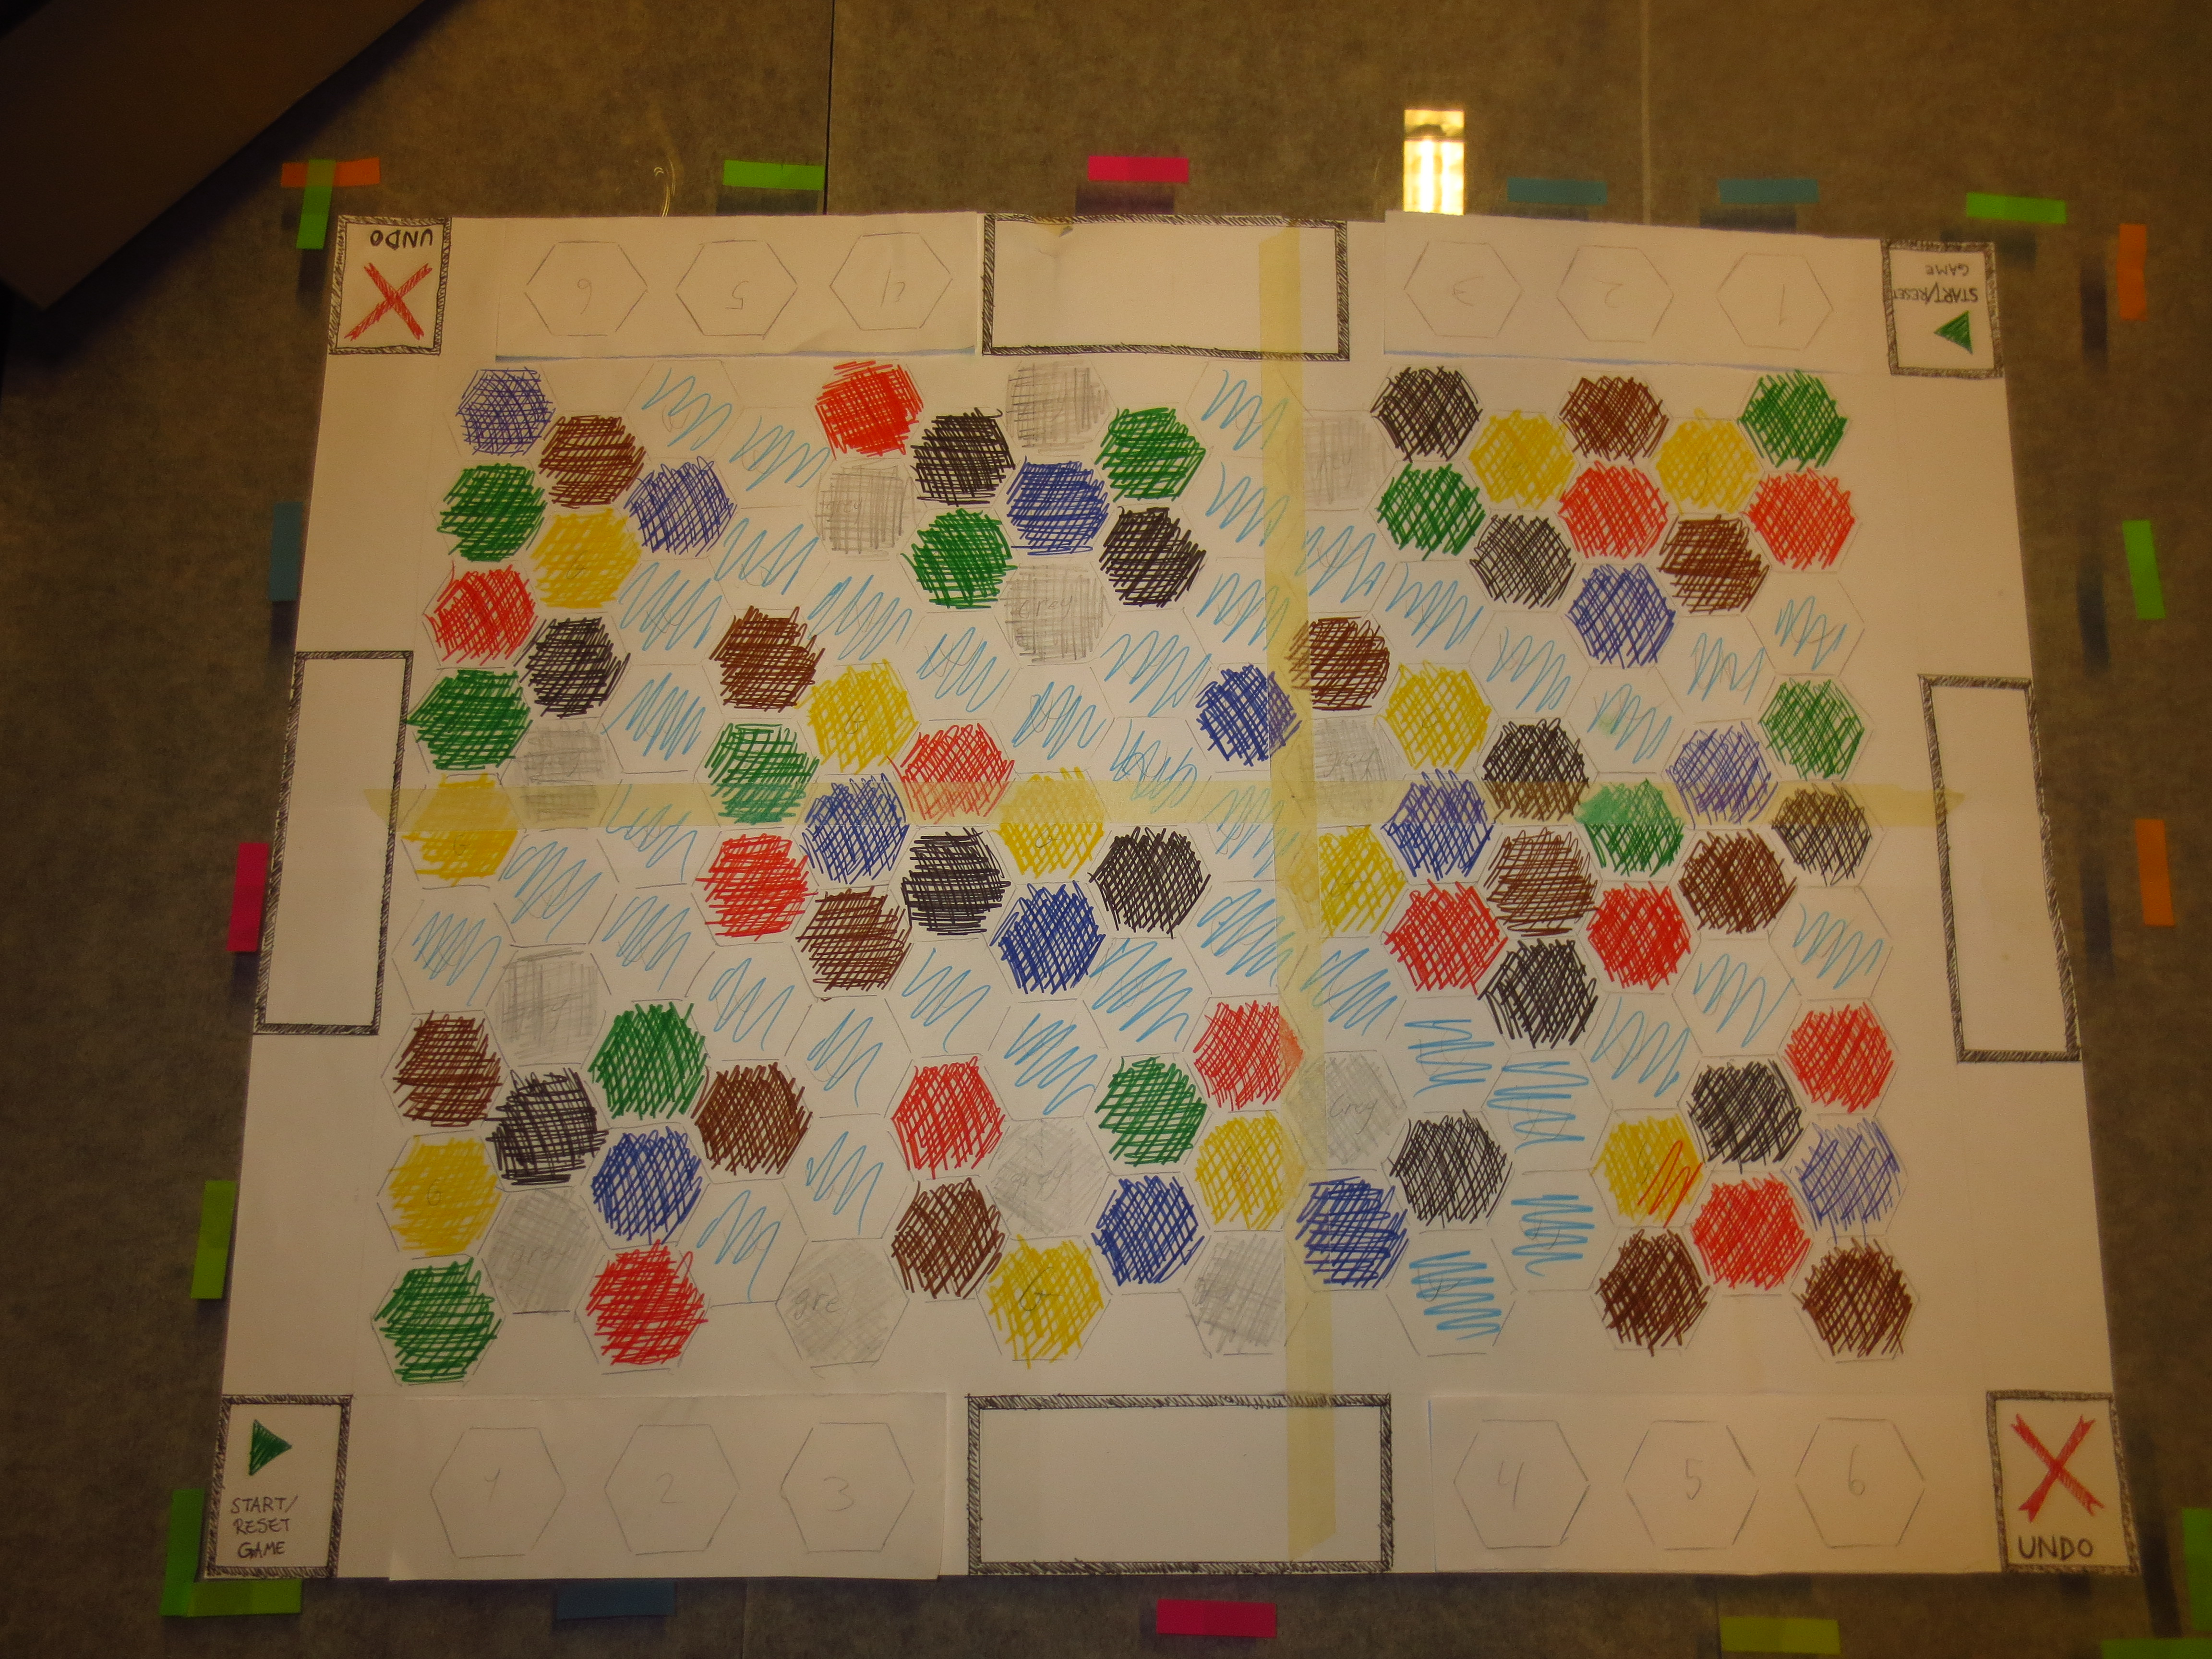
\includegraphics[width=0.9\textwidth]{IMG_0001}
\caption{The Lo-Fi board}
\end{figure}

After defining the initial design, a lo-fi test was conducted to test whether the areas of interest were large enough, the defined gestures were easy to perform, and if the increased size had any effect on the gameplay. We also wanted a first outside opinion of the game without the terraforming pieces.

\subsection{Procedure}
For the lo-fi we had three participants: Two female participants and one male, aged 20-25. 
They were all familiar with the game Terra Mystica, so they did not need to learn the game first. They only played two rounds, since one of the key points of the test was to learn if the gestures and the areas were appropriate. 

The participants were introduced to the Lo-Fi board, by the primary interviewer who also acted as the "program", about how the gestures worked and where they worked. They then played two rounds of the game, with some functions removed since they had no effect when only playing two rounds. During the game they commented out loud, which was noted down by the secondary interviewer who also noted down their reactions and behaviour. 
After the game they were asked some questions in a loosely structured group interview. 
The whole test was filmed.

\subsection{Results} 
The participants all had a little bit of trouble remembering to do the terraforming gesture in the beginning, but they were all pretty sure that with a little more playing it would come naturally. One female participants said: \textit{” I think it comes by itself when you play the game some more.”}. They also mentioned that it might be easier to remember to do the "start of turn"-gesture if the non-interactive areas of the board lit up in the colour of the currently selected player, as another female participant said: \textit{” I think it would help with some light or something like that”}.


They generally liked the bigger board, since this made the hexes and other touch areas bigger, but they did also mention that for short people, it might be a problem to reach the other end of the board. The male participant said: \textit{"I think it is easier with touch control and such, if it was the normal board it would have been a bit harder for me to place my fingers on it"} while one of the female participants said \textit{"It’s just [that] small people aren’t allowed [to stand] at the ends of the table"}.

The participants were curious to why the buildings, their placements and their upgrades were not digital like the terraforming. They then made the guess themselves that reducing the use and amount of game pieces further would remove some of the tangibility they like about the game. They mentioned that the augmented version made terraforming and building seem like very different actions to execute, and a way to make them seem more alike would be to also make touch interactions with the board when you were about to place building pieces.

The personal player input area could be utilised better. Maybe it could indicate income or victory points or just indicate whenever it is your turn. 

The conclusions of the lo-fi test are that the gestures are easy to do and the areas of interest are large enough. The increased size of the board did make it harder for smaller players. The next step is then to discern if the program will be able to recognise the gestures. 

\section{Board interface}\label{sec:BoardInterface}
\begin{figure}
\centering
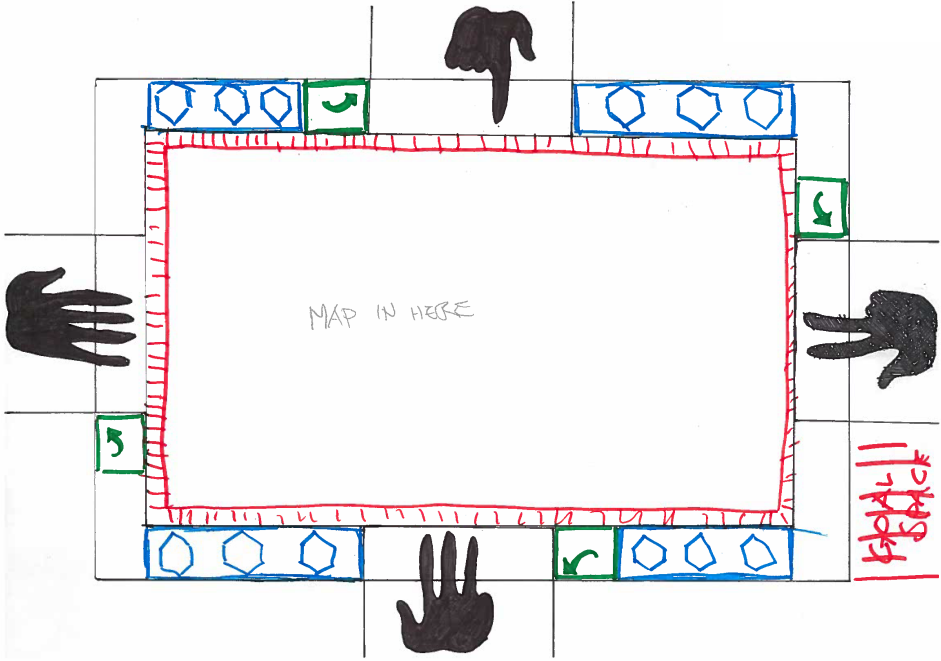
\includegraphics[width=0.9\textwidth]{sketchGUI}
\caption{Sketch illustrating the interface}
\label{fig:sketchGUI}
\end{figure}

The board interface itself should resemble the Terra Mystica Board to some extent, as shown on Figure~\ref{fig:sketchGUI}. The following elements should be on the board in the minimum implementation:
\begin{itemize}
\item A map consisting of hexagonal tiles, varying in colour. By default, they will be arranged like the original game board, but all non-river tiles should be able to change colour.
\item Four areas (marked by the hand icon on Figure~\ref{fig:sketchGUI}), where the players can indicate through gestures that it is their turn.
\item A space showing the global power actions which can only be taken once per round by any player. These are marked on Figure~\ref{fig:sketchGUI} in blue. In the minimum implementation, these are not interactive. However, as a further iteration, they can be made interactive, so that it is visible whether the action has been used or not without using tokens.
\item A victory point counter surrounding the map, shown as a red border on Figure~\ref{fig:sketchGUI}. In the minimum implementation, this is not interactive, and the points each player has accumulated must be shown using tokens, as in the original game. A further iteration to this could be to instead manage the points digitally, either by touching the point border itself, or adding add/subtract buttons at the edge of the board.
\item A space where the global goals for this round can be placed. These are managed using game pieces.
\end{itemize}

The following are not required for the minimum implementation, but can be added if time allows:
\begin{itemize}
\item Some undo buttons, marked on Figure~\ref{fig:sketchGUI} in green. These should be interactive, in case a players makes an incorrect action.
\item Detection of building placement, allowing the program to see when power should be offered to another player. The interface could then indicate that power needs to be offered, and in an ideal implementation, how much power. This would require shape recognition of the game pieces.
\item The empty spaces around the edge of the board could be coloured in the currently selected player's colour. This way, it would be visualised whether a player needs to indicate that it is their turn or not.
\item A space showing information about the players, such as race, colour, points, power, etc.
\item An area to place unused building pieces.
\item A space keeping track of the cult track, showing how many points each player has with the different cults.
\end{itemize}

\section{Requirement specifications}\label{sec:ReqSpec}
The following is the specifications of the usability- and software-based requirements needed in order to to design, build and program the interactive board for Terra Mystica. Note that not all of these are necessary to implement in the minimum implementation version of the product, as seen in this project. \todo{Add a reference here to the relevant section in final product}

\begin{enumerate}
\item On each of the four sides of the board, there needs to be an area where players can place a hand showing 1-4 fingers, indicating which player wishes to take their turn. The program must be able to read whether one, two, three, or four fingers have been placed on one of the player selection areas. The player with the corresponding amount of fingers as their gesture should then be selected.
	\begin{enumerate}
	\item Each of these four players must have a corresponding terrain type, represented by a colour.
	\item This must be successful 90\% of the time, as the type of tile placement depends on the player selected.
	\end{enumerate}
\item In the middle of the board, there should be a map consisting of 112 hexagonal tiles. On a player's turn, the program must be able to detect when a tile is selected for terraforming - that is, when a player places three fingers on the tile in question. This tile must then change to the terrain type of the last player who was selected.
	\begin{enumerate}
	\item This must be successful 90\% of the time. It is crucial that the program can tell the difference between placing a game piece on the board, and having the player select a tile via the three finger input. Depending on the efficiency of the program’s BLOB extraction, this might cause misunderstandings from the program.
	\end{enumerate}
\item In case of misplacement of terraforming, the program must be able to detect the use of an undo-button, which should be done with the same gesture as with the terraforming, but instead of doing the gesture on the map, the gesture is done on a visible button, which will be placed near the border, separate from the map.
	\begin{enumerate}
	\item This must be successful 90\% of the time.
	\item The undo-buttons area of interest needs to be secluded from the other areas of interest, so it can not accidentally be interacted with. 
	\end{enumerate}
\item In the game, there are actions which all players can take, but they can only be taken once per round. In the analogue game, a token is placed on the icon for the action when this happens. For the minimum implementation, this does not need to be managed digitally. However, there should be spaces on the board showing the different actions, on which the players can place tokens in order to remember which actions are already taken. There are six of these actions in total. All of these actions should be represented on the board twice; once on each side of the board, so that they are reachable by all players. This is shown in Figure \ref{fig:sketchGUI}, where the actions are the blue areas. 
	\begin{enumerate}
	\item A further implementation which is optional is to make the actions managed digitally. When an action is used, the player must select the action they wish to use by doing the same gesture as when terraforming. Doing this should toggle the action on and off. When the action is turned off, a cross should appear on the action area, showing the players that the action can now not be used.
	\end{enumerate}
\item The digital board should have a point counter. That is, a border around the board consisting of 100 tiles numbered 1-100. The red border on Figure~\ref{fig:sketchGUI} shows its placement. This border should not be managed digitally, but the players should be able to move a coloured token representing themselves from tile to tile, visualising how many points they have. The program should ignore the tokens placed on this border.
\item The board should have a space where the players can place the game pieces that represent the game goals. This space should not be interactive. This space is represented as the red space to the side on Figure \ref{fig:sketchGUI}. These are goals that either apply to only a single round, or to a whole game. Just as with the point counter, the goals should not be managed digitally, but just be covered with game pieces when they are not important.
	\begin{enumerate}
	\item Another optional implementation is to make the goals digitally covered. This could be done by allowing the players to hide them by pressing the goals.
	\end{enumerate}
\end{enumerate} 
%!TEX root = ../master.tex
\chapter{Implementation}\label{ch:implementation}
Our development chapter. \todo{We describe Rear Infused Illumination, and add all theory we have on the things mention if RID - for example BLOBs, contrast, illumination and so on.}

\section{Rear Diffused Illumination} \label{sec:RDI}
The interaction on the game board table will be based on rear diffused illumination as described in Multi-Touch Technologies \citep{multiTT}. As shown in figure ((ref project sketch)) this means we are going to make inputs in the augmented board game via having it recognise the touch of the board as BLOBs shown in IR light. This is because of a camera beneath the table's surface that observes a change in the contrast shown in IR light. 
For this to work, the table's top surface, made of transparent material, needs a diffuser material just above or beneath it in order to diffuse the light. Infra-red light then needs to be shone on it from beneath the surface. When the glass is pressed from above the surface by an object, that part of the surface reflects more light back which will be captured by the camera as a BLOB.
\begin{figure}[!h]
\centering	\includegraphics[width=0.5\textwidth]{sketchAugmentedBoard}
\label{Fig:sketch} \caption{An sketch of our RDI table.}
\end{figure}

Choosing such a solution has it's advantages and disadvantages. First of all, there is no need for a compliant surface or soldering for a LED frame, since we are using a diffuser in order to reflect the IR-light coming from below. The illuminators for that can be bought ready to go, so there is no need to build them. A disadvantage comes from the RDI having difficulties with getting even illumination, since the IR-lights might cover the table's surface completely. This can result in false BLOBs and BLOBs of lower contrast, which will challenge the software's detection of the real BLOBs.

\section{Physical Design} 
\begin{figure} [!h]
\centering 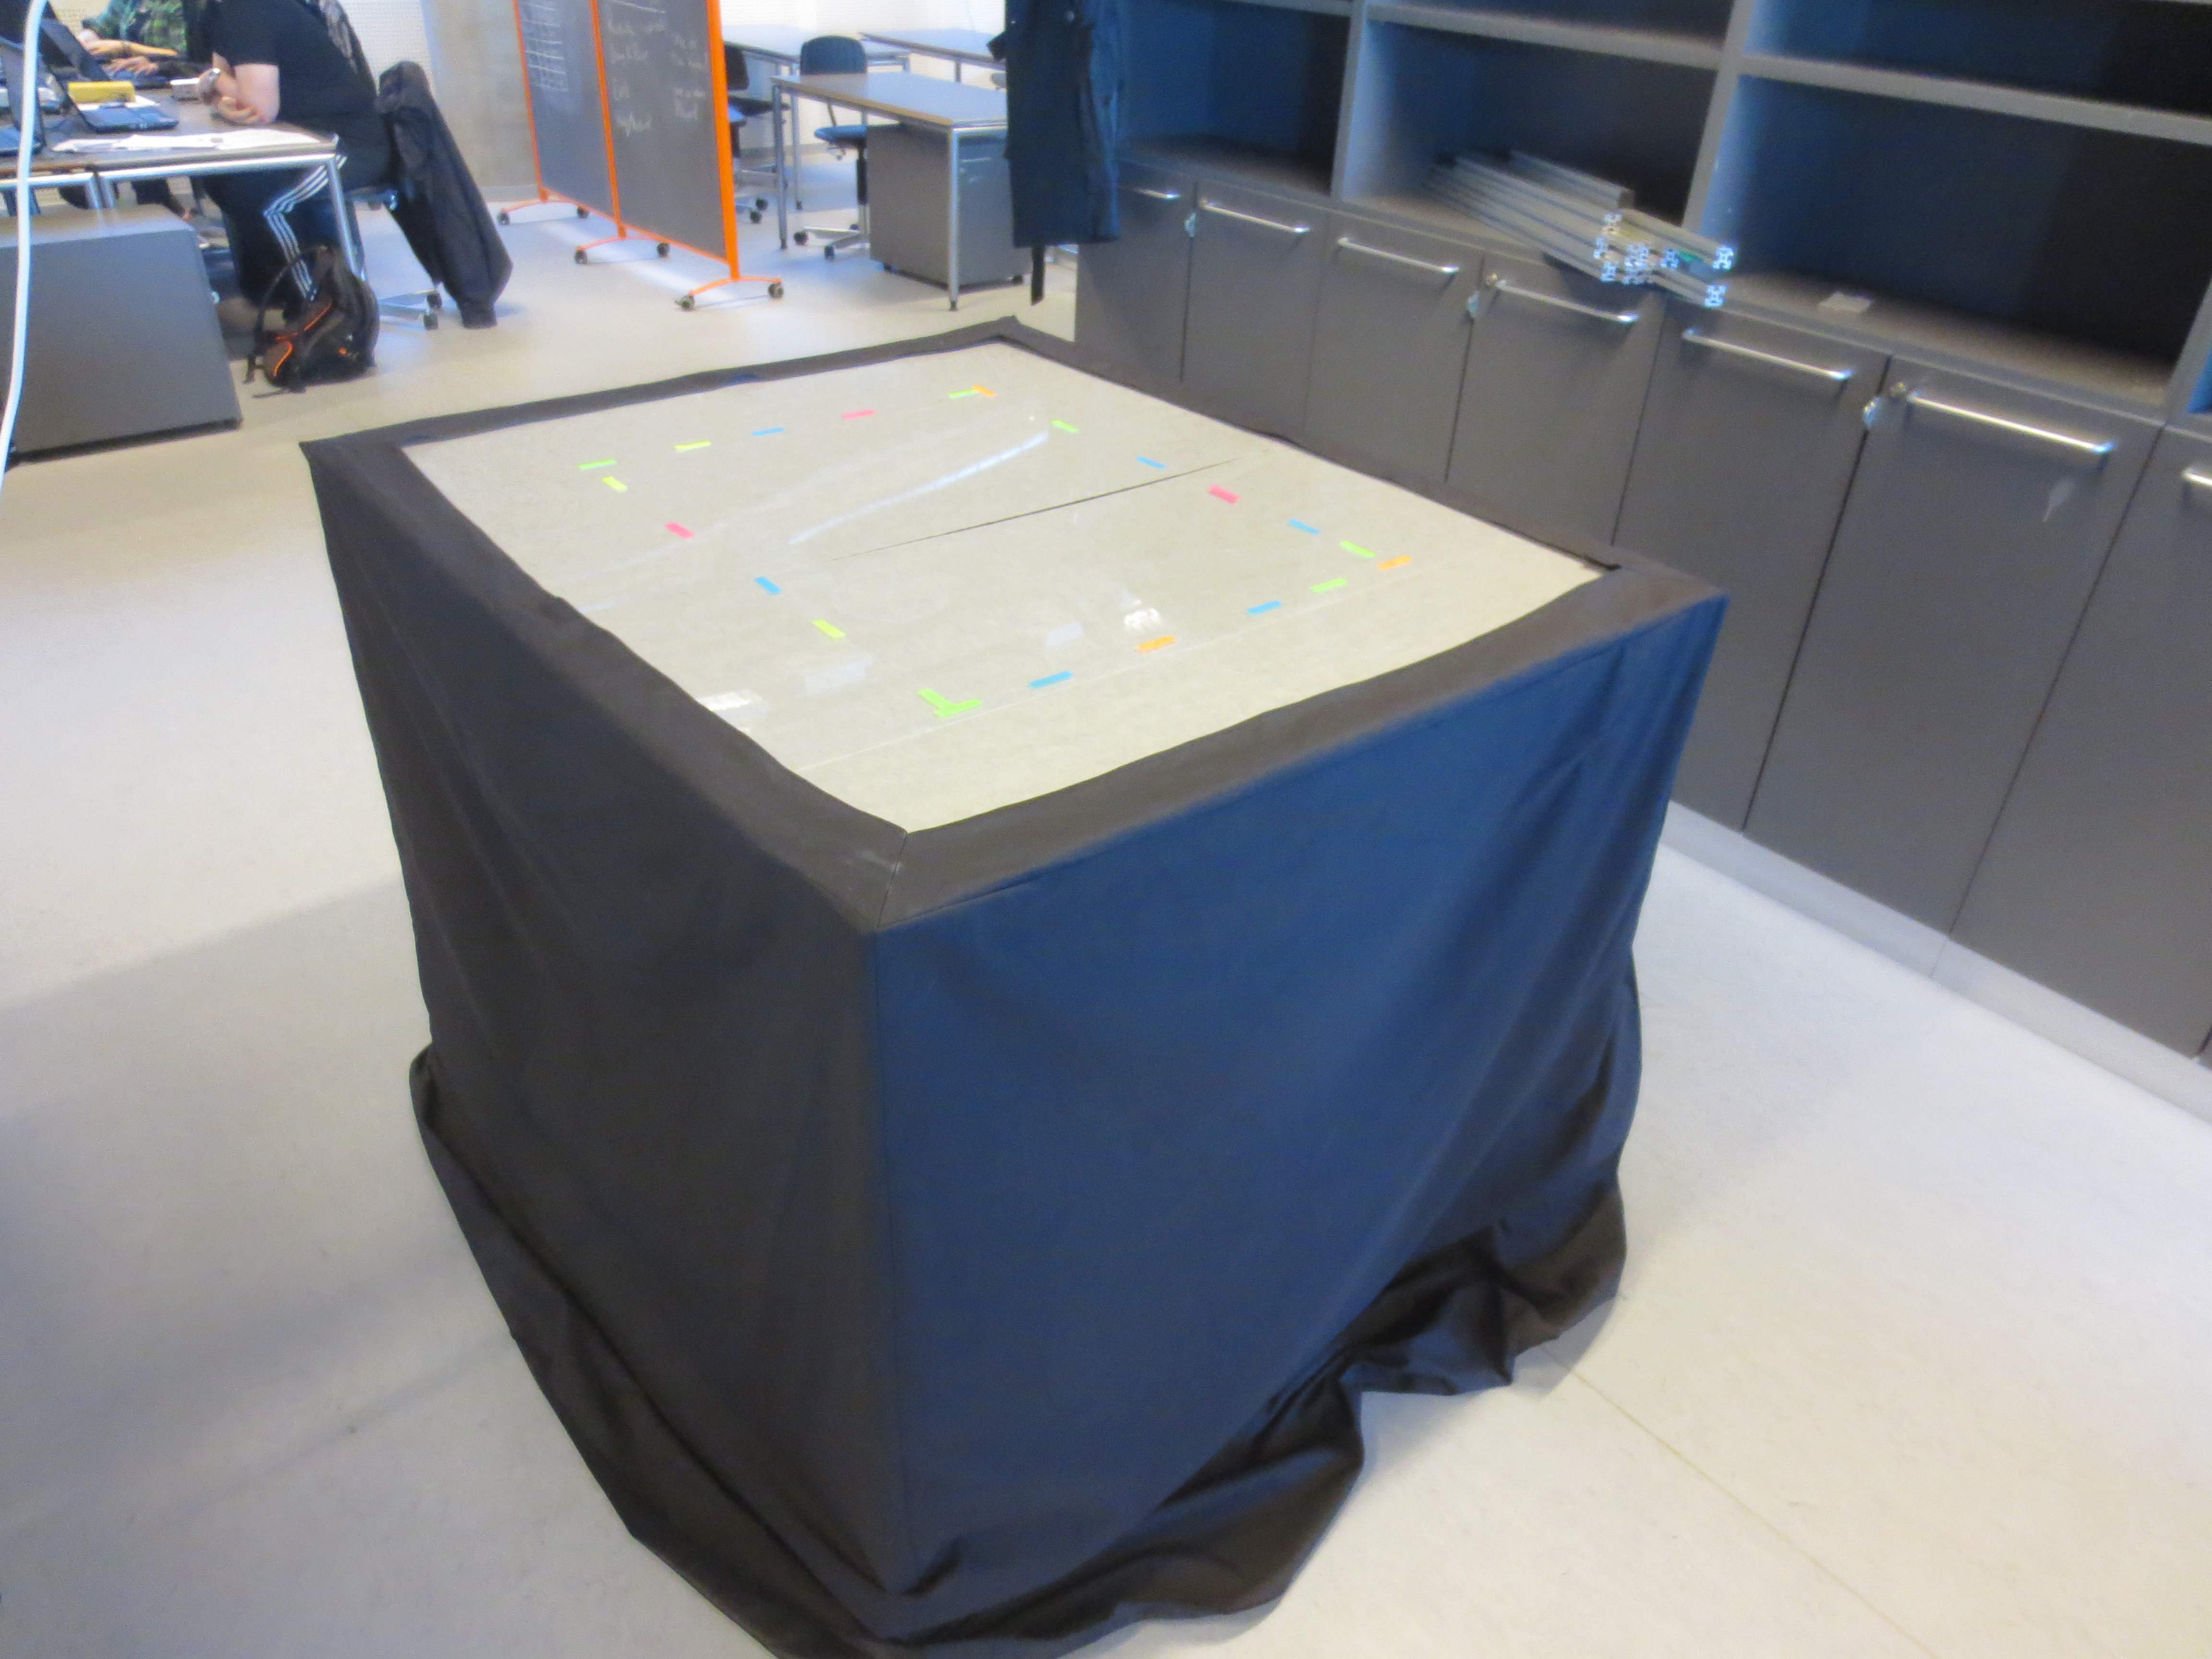
\includegraphics[width=0.5\textwidth]{Table}
\label{Fig:Table} \caption{The touch table}
\end{figure}
This section will describe the physical aspect of our product.
We have assembled a touch board, made with a acrylic glass top and IR lamps below. Underneath the surface of the top is a short-throw projector so we are able to project images on the table. Additionally we have a webcam with an IR filter placed at the very bottom of the table, so we are able to detect, what is happening on the table surface. This is thanks to the reflected IR light, as explained in section \ref{sec:RDI}.

The outer frame of the table is constructed from 3 different lengths of aluminium rods, giving the table a final size of 120 x 102 x 89 cm.
After the outer frame of the table was assembled, a cloth cover was made for the table. This was done by a member of the group, who sewed the cover together and made it to fit the table. \todo{who made it is irrelevant. rather write why we use a cover}To be able to test the interior, diffusing material was needed on the acrylic glass top. Baking paper was chosen for this job\todo{please describe why.}. The baking paper was attached on the bottom of the acrylic glass top, meaning that the user wouldn't be able to feel the baking paper when they interact with the board. 
With the exterior finished, it was time for the interior to be constructed. The positions of the electronics were decided and the interior was build, based on what gave the best results. 

During the construction of the table, a few problems were encountered. One of the problem encountered was that the baking paper did not sit tight against the acrylic glass and was slowly falling down. This gave us problems when trying to reflecting IR light from it. The problem was fixed by taping the baking paper to the acrylic glass with duct tape. 
Another problem that was encountered was that some smaller rods were needed to construct the interior. This problem was easily solved by cutting the rods cut to size. 

\section{Image Processing}
To facilitate user interaction, a software module is needed to analyse a video input and recognize specific features and changes in it over time. There are two main criteria for this software. It needs to:
\begin{itemize}
\item Recognize specific finger touches.
\item Recognize specific game pieces.
\end{itemize}

To do this, BLOBs need to be extracted from the video input through segmentation. Since it is difficult to create a uniform surface of reflected IR-light, it might be necessary to apply a filter to the input before segmentation. Furthermore, since this is a video feed rather than a static image, changes in illumination may need to be accounted for as well. This leads to a four-step solution for processing the video input:
\begin{enumerate}
\item Prepare video frame for segmentation (Pre-segmentation).
\item Segment image (Segmentation).
\item Remove noise from the segmented image (Post-segmentation).
\item Analyse BLOB(s) (BLOB-analysis).
\end{enumerate}

\subsection{Segmentation methods}
There are several methods for segmenting images. Relevant methods are discussed in this section. Since this project deals with video as opposed to static images, a single threshold with a fixed threshold value is not useful. The hardware setup uses Rear Diffused Illumination with infrared light sources, and an  infrared filter on a web camera. This should create an ideal image for segmentation using an automatic global thresholding method. This method makes use of the histogram of an image to identify the most optimal threshold value\citep{Moeslund2012c4}. In an ideal image, the histogram will have two distinct 'mountains' of pixel values, that is to say, there will be two groups of pixels that, within each group, have a similar brightness while at the same time the groups themselves are isolated from each other. In the case of this project, the image produced should have bright spots where the board is touched, on a dark plane which is to be considered the background. The software then needs to identify an optimal threshold value between these two groups. One such method, is to evaluate the Figure~\ref{eq:otsu} for each brightness value in the histogram. The result with the lowest value is then selected.
\begin{figure}[h]
	\begin{align}
	C(T)&=M_1(T)\cdot\sigma_1^2(T)+M_2(T)\cdot\sigma_2^2(T)
	\end{align}
	\caption{$M_1(T)$ is is the number of pixels left of $T$ and $M_2(T)$ is the number of pixels to the right. $\sigma_1^2(T)$ and $\sigma_2^2(T)$ is the variance of the pixels to the left and right repsectively \label{eq:otsu} \citep[p. 61]{moeslund_introduction_2012_chapter_5}}
\end{figure}


%!TEX root = ../master.tex
\chapter{Final Prototype}\label{ch:finproduct}
The following chapter contains a description of the state of the prototype, at the end of the project period.

\section{Physical prototype}
The table is constructed by aluminium extrusions, measuring 120 x 102 x 89 cm. A shelf is located on the internal side of the top frame, which is used to hold a 3 mm acrylic glass plate. The underside of the glass is covered in a single layer of baking paper. This acts as the diffusion material in the RDI setup, as well as the screen for the short-throw projector.

In the bottom of the table are extrusions, which hold the rest of the RDI setup and the projector. The camera is placed at the bottom of the table, so that the area of sight is larger. The projector is placed to one side of the table, as this makes the cone of projection land centrally on the screen. The IR lights are placed 30 cm into the air, by mounting them on top of extrusions. This height is optimal, as the camera can detect more, the closer the lamps are to the screen. However, the closer the lamps are to the screen, the smaller the cones are of infra-red light.  Furthermore, if the lamps were to be placed higher, the extrusions they were mounted on would then start blocking the projector, making parts of the screen not viewable by the users. In order to contain the IR light inside the table, a black cloth baffle is placed around the sides of the table.

A computer runs the software and is connected to the camera and projector. The camera acts as input for the software, and the projector shows the output on the screen.

\section{Digital prototype}
The prototype displays a recreation of the Terra Mystica board and includes the following graphics:
\begin{itemize}
	\item The hexagonal tiles in the seven different colours, plus the river tiles
	\item An inner frame around the board tiles, which is used to track each player's amount of victory points.
	\item An outer frame, which contains a table with instructions on how to score victory points at the end of each round and at the end of the game. It also contains an undo button and buttons for actions that can be taken by only one player each round.
\end{itemize}

\subsection{Interactive elements}
The tiles are interactive, as the game's primary interaction with the board is terraforming. Each tile is independently interacted with, and can be changed to the colour of the current player, using hand gestures. In the original game, it costs different amounts of resources to change different colours, depending on the colour of the player. The table does not manage this, and relies on the players managing the resources required themselves.

When a player starts their turn, they must make a gesture, so the system knows which colour to use if the player wants to terraform. Since the low amount of lamps used cause the middle area of the board to be more illuminated, and thus more responsive, than the outer edges, these gestures are done in the middle, as opposed to in the designated areas, as per the original design. In order to make the player selection more reliable, paper hands are given to each player to be used instead of their actual hands.

\subsection{Non-interactive elements}
The victory point tracker is not an interactive piece of the board. Instead, it is a static graphic, where each player has a game piece placed on their current number of victory points.

The outer frame also includes two undo buttons, placed in opposite corners, which was meant to give the players the ability to revert the last action taken. However, this is not implemented because of time constraints.

In the two other corners, an area displaying  the goals is placed. This is described with images illustrating what players will get victory points for in each round. Images illustrating what players score victory points for in the end of the game are also in this area. In the original game, this table can have random objectives for each round, but in the digital version, it is a static image used as a place holder.
%!TEX root = ../master.tex
\chapter{Code Overview}\label{ch:codeover}

\section{Point-processing}
There are three point-processing algorithms in this software; an RGB-to-Greyscale colour conversion algorithm, a normalization algorithm, and a thresholding algorithm. All of these make use of double-nested \texttt{for}-loops to apply their operations to each pixel as shown in Figure~\ref{fig:pointprocess}.
\begin{figure}[!h]
\begin{lstlisting}
for (int y = 0; y < src.rows; ++y)
{
	for (int x = 0; x < src.cols; ++x)
	{
		//Code here...
	}
}
\end{lstlisting}
\caption{Basic point-processing algorithm. \label{fig:pointprocess}}
\end{figure} 

The RGB-to-Greyscale algorithm creates an 8-bit single-channel image and then maps the mean of the RGB-values of the input image pixels to the output like shown in Figure~\ref{fig:rgb2gray}

\begin{figure}[!h]
\begin{lstlisting}
output.at<uchar>(y, x) = (src.at<Vec3b>(y, x)[0] + src.at<Vec3b>(y, x)[1] + src.at<Vec3b>(y, x)[2]) / 3;
\end{lstlisting}
\caption{RGB-to-Greyscale operation.\label{fig:rgb2gray}}
\end{figure}

The normalization algorithm finds the maximum and minimum pixel values of the input image using an OpenCV function. It then processes each pixel to normalize them to a new maximum and minimum using the operation shown in Figure~\ref{fig:normalize}.

\begin{figure}
\begin{lstlisting}
output.at<uchar>(y, x) = floor((src.at<uchar>(y, x) - min) * (newMax - newMin) / (max - min) + newMin);
\end{lstlisting}
\caption{Normalization of a pixel. \label{fig:normalize}}
\end{figure} 

Finally, the thresholding algorithm determines whether a given output pixel is white or black based on the if-else statement that is shown in Figure~\ref{fig:threshold}.

\begin{figure}
\begin{lstlisting}
if (src.at<uchar>(y, x) >= threshold)
{
	src.at<uchar>(y, x) = 255;
}
else
{
	src.at<uchar>(y, x) = 0;
}
\end{lstlisting}
\caption{Thresholding. If the pixel value is above the threshold, make it white. Else, make it black.\label{fig:threshold}}
\end{figure}

\section{BLOB extraction}
After segmentation, a grass-fire implementation scans the image for BLOBs. First, a nested \texttt{for}-loop like the one shown in Figure~\ref{fig:pointprocess} goes through every pixel to check whether any of them is white (i.e. part of the foreground). If this condition is met, the function will call another function, which contains the actual grass-fire algorithm. The grass-fire function is called with the position of the white pixel and the image itself as arguments. 
%!TEX root = ../master.tex
\chapter{Testing and Evaluation}\label{ch:testeval}
In order to evaluate the product and see to what extent it can be considered successful, a usability test will be conducted.

\section{Purpose of test}
The purpose of this test is to test usability and functionality of the product. The ISO 9241 \citep{ISO} standard defines usability as effectiveness, efficiency, and satisfaction of the user. Put more precisely, this means:
\begin{itemize}
\item Efectiveness: To what extent are the goals of the product achieved?
\item Efficiency: What resources (including time) are expended to achieve the goals?
\item Satisfaction: To what extent does the user find the system acceptable?
\end{itemize}
With these in mind, the test aims to clarify whether the product lives up to its test objectives.

\section{Test objectives}
Our problem statement is defined in Section~\ref{sec:ProblemStatement}. Based on this problem statement, it is important not only to test how well the program functions on a technical level, but also if the test participants still feel like they are playing the original board game, which will be tested on a level of satisfaction/acceptance.
The success criteria (Section~\ref{sec:SuccessCriteria}) and the system requirements (Section~\ref{sec:ReqSpec}) each add to the specifications on the technical and satisfactory  objectives of the test.
These parts together make up these test objectives:

\begin{enumerate}
\item Do the players still feel like they are playing Terra Mystica, when they are playing the augmented version? \todo{this might need specifications or a broader question}
\item Do the players feel like taking turns using the player selection gestures is an easy task, or a hindrance?
\item How well are players able to undo mistakes they did while terraforming?
\begin{enumerate}
\item Furthermore, does the player selection task live up to the requirement specification that it should be successful 90\% of the time?
\end{enumerate}
\item Do the players feel like the task of terraforming is easier to carry out than on the original board game?
\begin{enumerate}
\item Furthermore, does the terraforming task live up to the requirement specification that it should be successful 75\% of the time?
\end{enumerate}
\item How easily are players able to undo mistakes they did while terraforming?
\begin{enumerate}
\item Furthermore, does the undo task live up to the requirement specification that it should be successful 50\% of the time?
\end{enumerate}
\item Do the players feel that the augmented game board can replace the original game board?
\item How hindered is the pace of the game by the three actions each player can take (chose player, terraform and undo)?
\end{enumerate}

These objectives set the goals for the test, and help determine whether or not the test is successful. 

\section{Test methods}
The test methods used, their criteria and their measurement are meant to see if the test objectives are met.

\subsection{Test set-up}
The test will take place in a controlled setting, were nobody else than the test participants and testers will be present around the board while a game is taking place. The participants will be playing, and the testers will only act as observers who document the proceedings, and helpers/guides - in case the participants have any technical problems that prevent them from proceeding from the test.
The documentation of the test will be done by a tester filming the participants playing the game and a note-taker that also acts as the spokesperson for the testers.

\subsection{Participants}
The chosen test participants are typical users. They are within the target group, which is defined in Section~\ref{sec:TargetGroup}, meaning that they are experienced with board games. \todo{Write some more stuff when participants are selected}

\subsection{Procedure}
The test, when set up, will follow this procedure:

\begin{enumerate}
\item To begin with, the test guide will introduce the participants to the product, and explain the whole test procedure. The guide will have a script to read from, to make sure all participants are fully informed.
\item Once all participants understand the procedure, they will begin a game of Terra Mystica using the augmented board\todo{how long? we'll find out in pilot test}. During the introduction, they are encouraged to have dialogues with each other regarding their actions and thoughts as they play. This is inspired by the think aloud method addressed by Larsen \citep{TestingLecture}. The whole test is filmed by the cameraman. It is especially imortant to get footage of the participants' hands as they attempt to do gestures. It is likely that all of the typical tasks will be performed during this playthrough, but if not, the test guide will ask the test participants to attempt the ones they forewent.
\item Once the practical part of the test is over, the test guide will conduct a semi-structured group \todo{depending on amount of testers} interview, which the participants have been informed about during the introduction. The participants will be asked about how they experienced the augmented game, both in its own right, and in comparison to the original game.
\end{enumerate}

Once the test is done, the footage and notes from the test will be analysed and compared to the test objectives.

\section{Results}
text\todo{analysis and conclusion}\todo{remember to look at video to analyse delay of actions and how many tries before successful action}
%!TEX root = ../master.tex
\chapter{Discussion}\label{ch:discussion}

\section{Validity and reliability of tests}

\subsection{Validity and reliability of usability test}
When considering validity and reliability of the tests conducted one need to have some strategies to base it on. The strategies used in this section have been suggested by Creswell \citep{Creswell}.

Regarding validity they can be summed up to these points:
\begin{itemize}
\item Triangulate different sources of information and establishing themes.
\item When describing the findings it needs to be richly detailed, to represent the results as realistically as possible.
\item Clarify that the researcher is biased and self-reflect on the results.
\item Present the negative feedback and the feedback that does not fit with the majority to show that the different perspective have been considered.
\end{itemize}

As seen in section \ref{satisfactionResult} the results have been described thoroughly and present both the positive feedback that back up our problem formulation and the negative feedback that does not back it up. This is consistent whenever a new theme in the results is established. This gives the results some validity. In general throughout the test the testers have been encouraged to be as unbiased as possible but as it is not possible to put all ones own bias away the questions asked and the results ans themes reached are of course made on a basis of our bias of the product we have created. We have however as can be seen throughout the entire Chapter \ref{ch:testeval} considered all angles offered to us concerning the test results. This can be argued as giving our results a sufficient degree of validity. In hindsight, more could have been done to raise the degree of validity, as for example bring in test participants who were not fellow students and therefore wouldn't have the bias gained from the same study. 


Reliability deals with the test set-up and procedures. The points Creswell \citep{Creswell} makes on this topic can be summed up as follows:

\begin{itemize}
\item Check transcripts for mistakes after transcribing.
\item Make sure that the guidelines and procedures remain the same throughout the process.
\item Make sure all groupmembers are aware of the guidelines, procedures and results. 
\item Compare results reached independently.
\end{itemize}

There were not made transcripts of the final tests, since this would take too much time. Therefore we cannot argue for reliability on that point. However we kept to the same guidelines and script for all the tests which all the group members were aware of since different people conducted the tests. All the results were compared in the analysis in section \ref{subsec:analysis}. This all results in a high degree of reliability of our results. 

\subsection{On reliability in technical test and prototype}
This section will discuss the implications of calibration and bugs in the prototype use and testing. 
\subsubsection*{Calibration and reliability}
In order for the prototype to work, a lot of time has to go into setting it up, also called calibration. The IR lamps have to have the right angle and run for a while. The program has to be restarted at times, which also removes noise \todo{for some reason we don't know o.O}. Despite of all this, a lot of problems still remain as can be read below. This makes for poor reliability, as it is hard to test a prototype with such a fickle nature. The chance that you get the same parameters set up for testing twice are challenged and only overcome by several modifications and nudges.

While performing the technical test the people responsible kept a bug log as a tool to track common errors. The bug log can be seen in \ref{app:techTest} \todo{appendix missing} in its entirety.

The most common errors were ordered in tags: Neighbour Change (NBC), Shadow Threshold failure (SWT), and Area Detection Failure (ADF). 
\subsubsection*{Bug - NBC} 
NBC was a common error closely linked SWT, meaning that almost every occurence of NBC had a SWT bug as well. This could indicate that NBC wasn't really to blame, but SWT. Regardless, NBC pertains to the hexagon's centre and the centre of the convex hull (of the fingers trying to change it) are misaligned.
\subsubsection*{Bug - SWT} 
SWT was the most common area in the technical tests but also during the user evaluation tests. This bug has specifically to do with more than the fingers or hand being detected, such as parts of an arm. Furthermore, the bug can occur when a hand is hovering close to the board, but not touching it.
\subsubsection*{Bug - ADF} 
The ADF bug occurred most commonly when a player change was intended but a small-enough hull was made, resulting in a unintentional tile change.
\subsubsection*{Bug remedy}
Certain things could be done to remedy these bugs, such as:
\begin{itemize}
	\item Calibrating the threshold to avoid hovering elements, such as arms or close objects are not added as objects.
	\item Performing intelligent (with a learning rate) background subtraction to cancel out noise and ensure an easier thresholding. This would also reduce the calibration time.
\end{itemize}

\section{Further Implementation}
Aside from the product's minimum implementation requirements, it is possible to make further iterations, suggested in this chapter. These are based on the evaluation results from both the user test and the technical test, which is described in Chapter~\ref{ch:testeval}. The implementation suggestions are based in the results that are considered valid and reliable.

\subsection{Improvement of terraforming}
Although the implementation of an undo button was originally planned, it did not become a part of the current version. Participants of the usability test have voiced the need for such a function, as well as provided ideas to how such a function could be implemented (Section~\ref{satisfactionResult}). It could be a button, which is a visible part of the board's GUI, placed away from the game map. This button could revert the last terraforming action taken in the game. An algorithm for this function could be a stacking system that remembers previous actions, allowing the program to revert them, returning to previous states of the program. Another solution could be an expansion of the terraforming action. Anyone, regardless of whose turn it is, should then be able to change a tile to any type of terrain in the game through a multiple choice menu. This would help users undo mistakes by letting them change the tiles back to what the player originally intended or back to their original state. A possible problem with the multiple choice solution is its dependency on players' memory regarding what the terrain of the hexes originally were before the misplaced terraforming. 

\subsection{Improvement of taking turns}
Participants of the usability test had ideas how to improve the turn taking further, besides improve in its programming. They mentioned that instead of switching player by pressing a hand against the middle of the surface, one should be able to switch turns by interacting with an area specifically only for switching turns. This will require the diffuser to be more evenly illuminated, which could be done by adding more IR lamps, making the originally planned player selection areas properly illuminated and thus usable. Properly illuminating the diffuser would also make BLOB detection more precise in general, possibly allowing players to use their own hands more rather than paper templates.

\subsection{Turn specification}
Test participants also noted they would like to have a visible indication of whose turn it would be next, and an overview of the turn order at any given time. Which player has the next turn could for example be visible on the game's GUI by highlighting the player's personal area of the board, or by colouring the space not used on the board with the player's colour, in order to emphasise which player currently is in charge of the turn.
Regarding the turn overview, a solution to that could be an overview implemented as part of the board's GUI. Its placement could either be as a part of the board's global information, just like the game objectives, in which case it would have to be large enough for each player to observe it clearly, or in front of every player, giving them each a equal personal overview of the turn order. In addition, one could design the overview so each overview graphic had focus on the player's placement in the turn order. The latter solution's advantage is an easier overview for all players, since none would have to look at the turn order from an odd angle. However, the first solution's advantage is that it might take up less space than having an overview for each player.

\subsection{Digital race/faction card}\label{sec:DigiRaceFact}
As one test participant mentioned, a fully digital version of the board game is possible. One could implement a graphical representation of the faction card and the information that normally follows in the original version of the game. As the faction card is made digital, it can also undergo changes in the way it visualises rules and upgrade costs. This could be implemented by making the icons for the tasks interactable, making the user able to show and hide tool tips explaining the task. If that text would take up too much space, making the cards too large on the board, a design idea could be to make up a tool tip box, specifically for text, which would change depending on which part of the race card graphics were interacted with. Another thing a digital faction card can implement is the possibility to upgrade a player's terraforming or shipping tasks, making them more effective. In the original game, this is done by moving a physical marker on the faction board. The digital faction board could be designed so it would change an upgradeable part when interacted with, for example by pressing the relevant part of the card, which would upgrade it and change its graphic representation.

\subsection{Management of resources}
Several test participants disliked the physical management of resources (power, gold, workers and priests), which can be remedied by managing the resources digitally. This could have the added benefit of increasing the game pace. This digital management of resources could work with the digital faction board mentioned in Section~\ref{sec:DigiRaceFact}, with tool-tips explaining the resources in detail. The resources could either be interactive, so the users change their amount themselves, or it could happen automatically as users choose to upgrade, build, terraform, etc. If the latter solution is to be implemented, the following can be considered:
\begin{itemize}
\item \textbf{Income:} Depending on the player's buildings and their racial powers and upgrades, a specific amount of gold, workers, priests and power should be received after the beginning of each round. If the augmented board could register the buildings each player owns, it could use this information to give each player their resource income every round. 
\item \textbf{Power reminder, offer and receiver:} This implementation requires for the augmented board to recognise the placement of buildings, and to keep trace of which players the buildings belongs to. Every time a player places a building next to one belonging to their opponent, the program should remind the players that power must be offered, and specify how much power is supposed to be offered, depending on the value and placement of the buildings. This graphic reminder could for example either be shown in its own area of the interface, or be shown as a pop-up, which could reinforce its ability to remind the players of what they need to do.
\item \textbf{Cult tracking:} As the cult tracker originally is done on its own board, it normally is not a part of the main game board. This could be changed in the augmented version, as one could design it to be a part of the interface. This information could be shown graphically either by having a tracker looking like the original one, or a more simplistic version, which would show the level of progress each player has in each cult. When specific milestones are reached in the cult tracker, the board could notify the players of what they gain from the milestones. This tracker could also, like in the original version, show the priests sacrificed and take care of the progression on tracker automatically every time a player did anything in order to progress.
\end{itemize}
%!TEX root = ../master.tex
\chapter{Conclusion}\label{ch:conclusion}
Based on the results from the testing and evaluation of the prototype for the augmented Terra Mystica board, both usability-wise and technologically (Chapter \ref{ch:testeval}), an answer can be given to the problem statement from Section \ref{sec:ProblemStatement}.

\section{Problem Formulation}
The problem formulation is twofold:

\textit{“Can Terra Mystica become more usable through the use of a computer vision augmented board…”}

According to the results from this project, the answer is \textit{not at the prototype’s current state, but possibly in the future}. When testing the prototype, it became clear from the participants' usage that it slowed down the pace of the game because functions were not working efficiently. It was the terraforming and turn mechanics that took longer than in the original version of the game, which was caused by the users having trouble doing those actions. Despite this, some of the participants said they expected the actions not to be an hindrance at all if their functionality worked flawlessly. Some participants expected a faster pace of the game, if the augmented version had functions which took care of a player’s resource management. Furthermore, participants saw a potential in the augmentation interface design, since they believed its simplistic design would benefit new players, and that it could have a more explanatory GUI, which for the new players might increase the game’s usability. All this will require an improved version of the prototype. It should then be tested in order to see if those ideas do increase the game’s usability. This is why, may only in a later version make Terra Mystica become more usable through the use of a computer vision augmented board.\\
\\

\textit{“...while still maintaining the feeling of playing a traditional board game?”}

With the results in mind, the answer here is \textit{the prototype kept the players feeling like they still were playing a traditional board game, although the augmentation could change the game’s purpose}. The consensus between the participants was that they felt like they were playing the same game in both versions, despite the difference in how some actions in the game were executed. However, there were still participants who saw another change in the game’s purpose from the original to the augmented one. Some saw the augmented version as a simpler, larger, and clearer version of the two. Others saw the augmented board game as a more dramatic game to play, since instead of placing tokens for terraforming, you used your hands to do it. Additionally, some saw the two versions of the games as two ways of playing it, since one was by a large box you had to stand up to use, while light was shining from the board, and the other was a smaller, more tactile version, were you sat down and were closer to each other. In conclusion, the participants still felt like they were playing Terra Mystica, and it maintained the board game feeling, even though the different versions could represent different purposes of use.

\section{Success Criteria}
\textit{"The project must have gone through evaluations and iterations, based on relevant usability principles."}

The prototype was developed through multiple stages, first being tested as a paper mock-up. After this initial lo-fi testing, the feedback led to the second stage of development, which made use of the RDI setup for the use of terraforming. This stage was then tested with more participants, whose feedback led to establishing steps for further implementations of the augmented board game.\\
\\

\textit{"Augmentation technology must be utilised with Terra Mystica in such a way that it does not take away from the experience of the game but enhances it."}

In the usability testing of the prototype, many participants expressed positive interest in the board, when asked how they would respond if the prototype was developed into a fully implemented product. However, when asked if the prototype could replace the board game in its current state, the participants answered much more negatively, as technical issues and difficulties with RDI slowed the game’s pace and made hand gesture detection unreliable. Although some players reported that the simpler graphics of the augmented board was easier to get an overview from, others said the same from the more detailed tiles of the original board. Therefore, this success criterion is not fulfilled, with the prototype in its current state.\\
\\

\textit{"Implemented augmentation technologies should utilise computer vision to augment Terra Mystica"}

By making use of an RDI setup in order to detect gestures in the augmentation, the prototype removed the use of cardboard disks when terraforming. Instead it makes use of the player placing their hand on the table, in order to terraform and change turns. Therefore, this success criterion is fulfilled.\\
\\

\textit{"The accuracy and effectiveness of the image detection should be tested in a proper framework."}

The image detection implemented in the prototype was tested according to the framework described in Section \ref{subsec:techtest}, where accuracy, effectiveness, and overall efficiency of the system are tested. Appendix~\ref{app:techTest} documents the results of the testing carried out. However, whether it is a proper framework is debatable, as it is not built upon previous known methods of technical testing. Nonetheless, because of its defined procedural structure and clear display of data, this success criterion is considered to be fulfilled.
\bibliography{bib/mybib}
\label{bib:mybiblio}
\appendix
%!TEX root = ../master.tex
\chapter{Blueprints}\label{blueprint}
\begin{figure}[h]
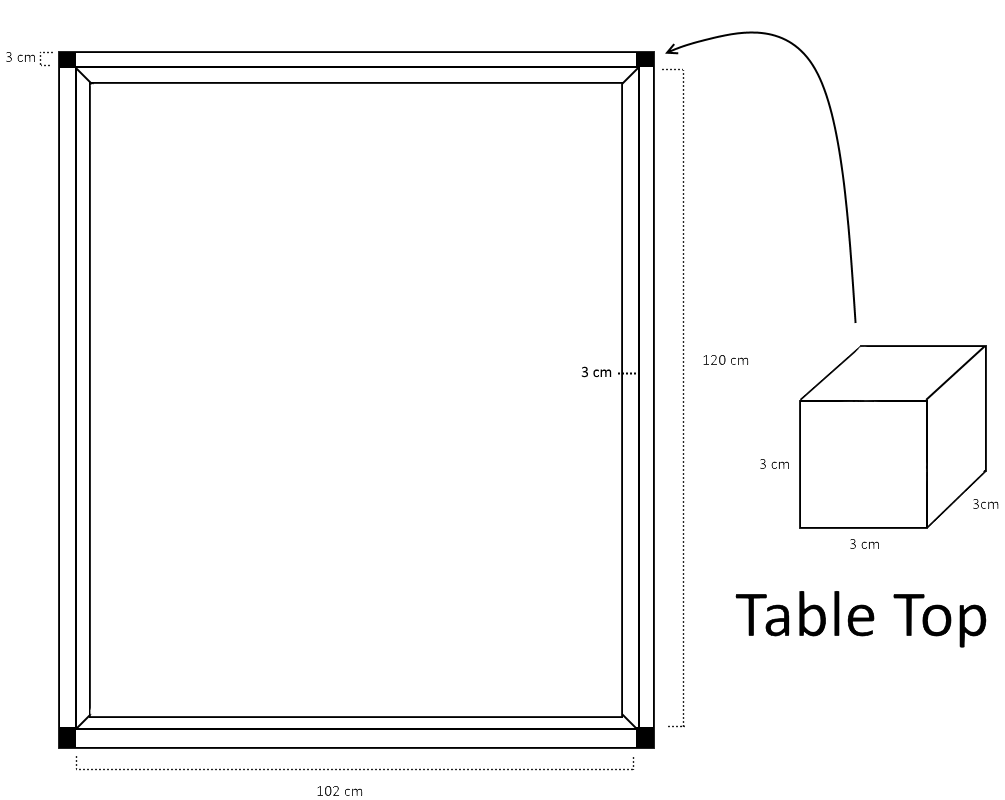
\includegraphics[width=\textwidth]{TableTop}
\end{figure}

\begin{figure}
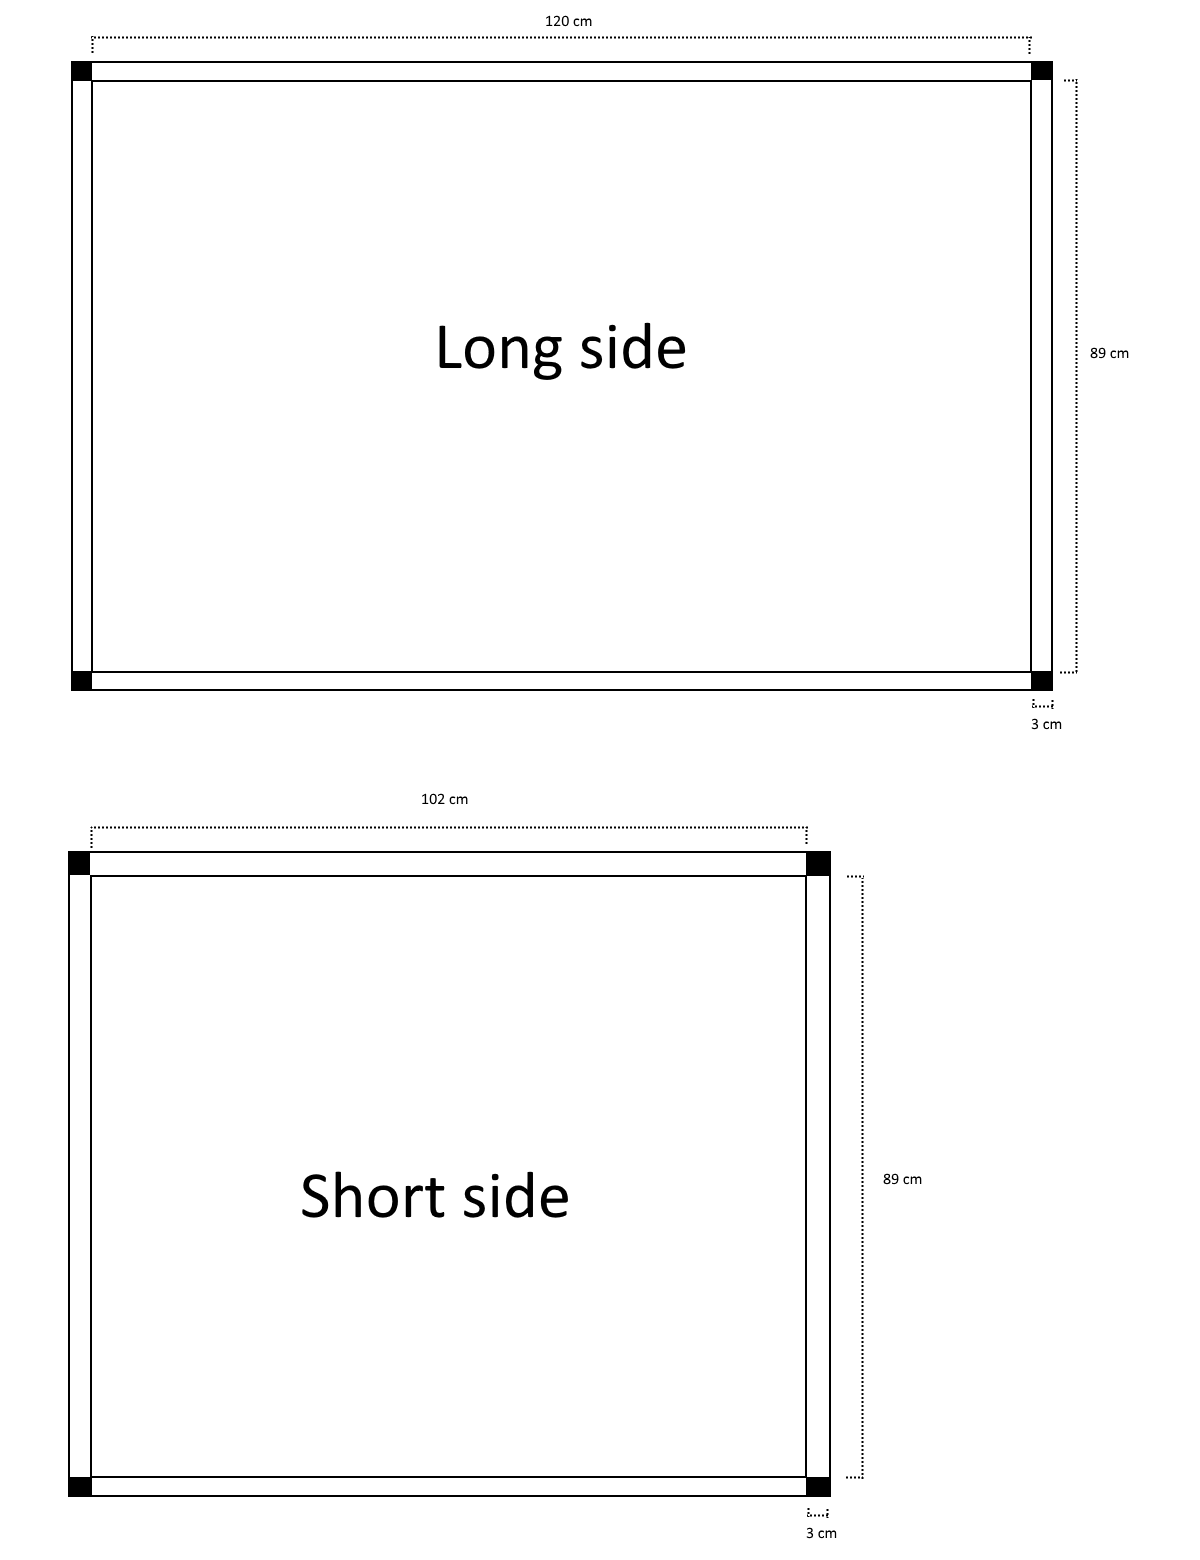
\includegraphics[scale=.5]{TableSides}
\end{figure}

\begin{figure}
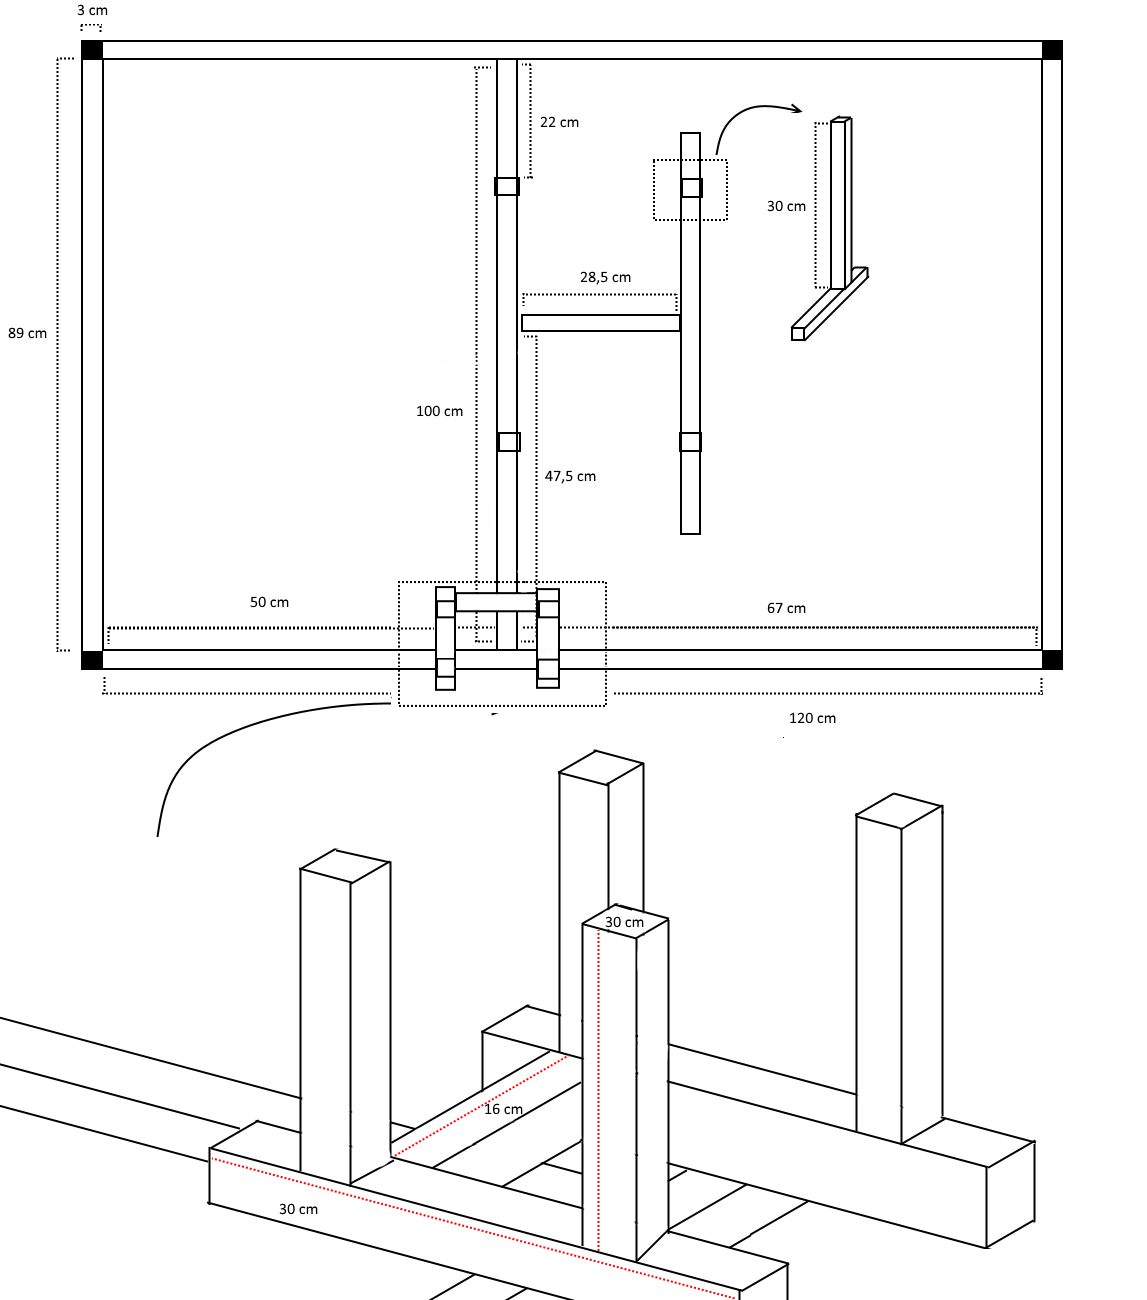
\includegraphics[scale=.5]{TableBottom}
\end{figure}
%!TEX root = ../master.tex
\chapter{Evaluation script}\label{ch:TestScript}
\section{Introduction to test}
(To the whole group)
Hello, and thank you all for agreeing to participate in our test. We have created a touch board table on which you can play the board game Terra Mystica. In other words, our product is a digitally augmented version of Terra Mystica.

You will start out by playing three rounds of the game on the [digital/analogue] version. While you play, you are encouraged to talk amongst each other about the game, and voice your thoughts. Once the three rounds are up, we will switch to the [digital/analogue] version, on which you will also play three rounds.

When you have played the two games, we will hold a short interview where you will be asked questions about your thoughts towards the augmented game. In this interview, you will also be asked to compare this version to the original game.

\section{Introduction to Terra Mystica rules}
For the purpose of this test, you will play a simplified version of the game.


\section{Explanation of the analogue version}
[Assuming they have played the digital version first]
The analogue version is played the same as the digital version, except you do not do a gesture when taking your turn, and you terraform by placing a token of your own colour on the tile you wish to terraform, like this [show it]. The buildings you wish to place are place on top of this token, like this [show it].

\section{Explanation of the digital version}
[Assuming they have played the analogue version first]
The digital version is played the same as the analogue version, except you now need to register yourself every time it is your turn, like this [show it], and instead of placing the tile tokens, you instead terraform like this[show it]. You will still place the buildings like before [show it].

\section{Post-test interview}
The following are points which needs coverage. This means that they should be used for a semistructured interview (meaning that the interviewer can, at any time, ask the interviewee to elaborate), made up by the questions raised from the testing and from the following: 
\begin{itemize}
\item How did you think the augmented Terra Mystica compares to the original game?
\begin{itemize}
\item Do you still feel like you were playing the same game when you were playing the augmented version?
\end{itemize}
\item How did you experience the act of indicating that is was your turn? Did you experience it as easy or difficult?
\begin{itemize}
\item How is the experience of taking turns in comparison to when playing the original game?
\end{itemize}
\item Did you experience ease or difficulty when terraforming compared to the original game?
\item Do you think the augmented game can serve as a possible replacement for the original board?
\item How do you think the game's pace was affected by the augmentation? Do you think it was increased or decreased?
\end{itemize}




\end{document}
